\documentclass[12pt]{article}
\usepackage{longtable}
\usepackage{pdflscape}
\usepackage{graphicx}
\usepackage{tikz}
%------------------------------ Tikz Libraries ---------------------------------%
\usepackage{ifthen} % \ifthenelse{condition}{yes}{no}  
% \ifthenelse{1>2 \OR 3=3}{yes}{no}    \ifthenelse{1>2 \AND 3=3}{yes}{no}
\usepackage{pgfplots}
\usetikzlibrary{arrows,arrows.meta}
\usetikzlibrary{shadows, shadows.blur}
\usetikzlibrary{backgrounds,calc, chains,fadings, fit, intersections}
\usetikzlibrary{patterns, positioning, scopes, shapes, through} % through: a library which even has the command circle through
\usetikzlibrary{decorations, decorations.markings, decorations.pathreplacing, decorations.pathmorphing, decorations.shapes} %  need to load the (sub-)library for the particular decoration e.g. (decorations.pathmorphing for zigzag, coil) (decorations.shapes for triangles, crosses), (decorations.pathreplacing for braces, expanding waves) 
%-------------------------------------------------------------------------------%

%==========================  Middle & pointing arrows ==========================%
%-------------------------------------------------------------------------------%
% usage: \draw[->-] or \draw[->-=6pt red]
%-------------------------------------------------------------------------------%
\tikzset{
    ->-/.style args={#1 #2}{ 
        decoration={
            markings,
            mark= at position 0.5 with
                {
                    \fill[#2] (#1/-6.0,0pt) -- (-0.5*#1, #1/3.0) -- (0.5*#1,0pt) -- (-0.5*#1, #1/-3.0);
                    %\draw[thick, #2]  (-0.433*#1,#1/2) -- (0.433*#1, 0) -- (-0.433*#1,-#1/2);  % switch to 60 degree arrow
                },
        },
        postaction={decorate}
    },
    ->-/.default={7pt black}
}
%===========================  place tangential arrows ==========================%
%-------------------------------------------------------------------------------%
% usage: \draw[arrow] or \draw[arrow=0.5 7pt green 1] or 
% or \draw[arrow=0.5 7pt thick 2]  
%-------------------------------------------------------------------------------%
% usage: \draw[arrown={0.5}{7pt}{red,line width=1pt}{2}]
% the #3 in arrown can be compound properties 
%-------------------------------------------------------------------------------%
% other values for #4 is for latter externsion e.g. draw a star, a circle
%-------------------------------------------------------------------------------%
\tikzset{
    arrown/.style n args={4}{ 
        decoration={
            markings,
            mark= at position #1 with
                {
                    \ifthenelse{#4 = 1}{
                    \fill[#3] (#2/-6.0,0pt) -- (-0.5*#2, #2/3.0) -- (0.5*#2,0pt) -- (-0.5*#2, #2/-3.0);
                    }
                    {
                        \ifthenelse{#4 = 2}{
                            \draw[#3]  (-0.433*#2,#2/2) -- (0.433*#2, 0) -- (-0.433*#2,-#2/2);
                         }{}
                    }
                },
        },
        postaction={decorate}
    },
    arrow/.style args={#1 #2 #3 #4}{ 
        decoration={
            markings,
            mark= at position #1 with
                {
                    \ifthenelse{#4 = 1}{
                    \fill[#3] (#2/-6.0,0pt) -- (-0.5*#2, #2/3.0) -- (0.5*#2,0pt) -- (-0.5*#2, #2/-3.0);
                    }
                    {
                        \ifthenelse{#4 = 2}{
                            \draw[thick, #3]  (-0.433*#2,#2/2) -- (0.433*#2, 0) -- (-0.433*#2,-#2/2);
                         }{}
                    }
                },
        },
        postaction={decorate}
    },
    arrow/.default={0.5 7pt black 2}
}

%======================== middle arrow on every subpath ========================%
%-------------------------------------------------------------------------------%
% usage: \draw[decoration=arrows, decorate] (0,0) -- (1,1) -- (2,0) -- (3,1) -- (3,0) -- (2,-1);
%-------------------------------------------------------------------------------%
\pgfdeclaredecoration{addarrows}{draw}{
\state{draw}[width=\pgfdecoratedinputsegmentlength]{%
  \path [every arrow subpath/.try] \pgfextra{%
    \pgfpathmoveto{\pgfpointdecoratedinputsegmentfirst}%
    \pgfpathlineto{\pgfpointdecoratedinputsegmentlast}%
   };
}}
%\tikzset{every arrow subpath/.style={->-,draw}}

\tikzset{
    arrows/.style args={#1 #2}{
        every arrow subpath/.style={->-=#1 #2, draw,thick}, 
        decoration=addarrows, postaction={decorate}
    },
    arrows/.default={7pt black}
}

%======================= improved \appendarrow{}{}{} ===========================%
%-------------------------------------------------------------------------------%
% usage: \arrowdraw[]{6pt}{red}{path};   % the first optional argument specify the 
% properties of the path
%-------------------------------------------------------------------------------%
\newcommand{\arrowdraw}[4][thick]{
\tikzset{
    middlearrow/.style args={#2}{
        decoration={
            markings,
            mark= at position 0.5 with
                {
                    \coordinate (exy1) at (#2/-6.0,0pt);
                    \coordinate (exy2) at (-0.5*#2,#2/3.0);  % 3.0 adjustable 
                    \coordinate (exy3) at (0.5*#2,0pt);
                    \coordinate (exy4) at (-0.5*#2,#2/-3.0); % 3.0 adjustable 
                },
        },
        postaction=decorate
    },
    middlearrow/.default= 3pt
}
\draw[#1, middlearrow=#2] #4;
\fill[#3] (exy1) -- (exy2) -- (exy3) -- (exy4) -- cycle;
}

%=====================  get and use tangent of a curve =========================%
%-------------------------------------------------------------------------------%
% usage: \draw[tangent=0.5 tangent=0.6]
%         \draw[use tangent=2] (-1,0) -- (1,0);
%-------------------------------------------------------------------------------%

\tikzset{
    tangent/.style={
        decoration={
            markings,% switch on markings
            mark=
                at position #1
                with
                {
                    \coordinate (tangent point-\pgfkeysvalueof{/pgf/decoration/mark info/sequence number}) at (0pt,0pt);
                    \coordinate (tangent unit vector-\pgfkeysvalueof{/pgf/decoration/mark info/sequence number}) at (1,0pt);
                    \coordinate (tangent orthogonal unit vector-\pgfkeysvalueof{/pgf/decoration/mark info/sequence number}) at (0pt,1);
                }
        },
        postaction=decorate
    },
    tangent/.default=0.5,
    use tangent/.style={
        shift=(tangent point-#1),
        x=(tangent unit vector-#1),
        y=(tangent orthogonal unit vector-#1)
    },
    use tangent/.default=1
}

%==============================  Multiple arrows ===============================%
%-------------------------------------------------------------------------------%
% usage: 
%    \draw[blue] plot [smooth,tension=1]
%	 coordinates {(A) (1,0) (1.14,-0.6) (0.5,-0.5) (0.5,0.5) (1.5,0) (B)}
%[arrow inside={end=latex,opt={red,scale=1.5}}{0.1,0.2,0.3,0.4,0.5,0.6,0.7,0.8,0.9}];
%
%-------------------------------------------------------------------------------%
\tikzset{
	set arrow inside/.code={\pgfqkeys{/tikz/arrow inside}{#1}},
	set arrow inside={end/.initial=>, opt/.initial=},
	/pgf/decoration/Mark/.style={
		mark/.expanded=at position #1 with
		{
			\noexpand\arrow[\pgfkeysvalueof{/tikz/arrow inside/opt}]{\pgfkeysvalueof{/tikz/arrow inside/end}}
		}
	},
	arrow inside/.style 2 args={
		set arrow inside={#1},
		postaction={
			decorate,decoration={
				markings,Mark/.list={#2}
			}
		}
	},
}

%===============================  Feynman diagrams =============================%
%-------------------------------------------------------------------------------%
% Hatree loop usage: \draw (0,0)  to[in=-50,out=-130,loop] (0,0); 
%-------------------------------------------------------------------------------%
\tikzset{
    bareG/.style args={#1 #2}{ 
        decoration={
            markings,
            mark= at position 0.5 with
                {
                    \fill[#2] (#1/-6.0,0pt) -- (-0.5*#1,#1/3.0) -- (0.5*#1,0pt) -- (-0.5*#1,#1/-3.0);
                },
        },
        postaction={decorate}
    },
    bareG/.default={6pt black}
}
%-------------------------------------------------------------------------------%
\tikzset{
    boldG/.style args={#1 #2 #3}{ double distance=#2, color=#3, 
        decoration={
            markings,
            mark= at position 0.5 with
                {
                    \fill[#3] (#1/-6.0,0pt) -- (-0.5*#1,#1/3.0) -- (0.5*#1,0pt) -- (-0.5*#1,#1/-3.0);
                },
        },
        postaction={decorate}
    },
    boldG/.default={6pt 0.3mm black}
}
%-------------------------------------------------------------------------------%
\tikzset{
    bareU/.style n args={3}{#3,
	decorate,decoration={snake,amplitude=#1, segment length=#2, pre length= 0.4*#1, post length=0mm}
	},
	bareU/.style args={#1 #2 #3}{color=#3, semithick,
	decorate,decoration={snake,amplitude=#1, segment length=#2, pre length= 0.4*#1, post length=0mm}
	},
%	bareU/.default={.8mm 0.25cm black}
	bareU/.default={.4mm 0.15cm black}
}
\newcommand{\bareU}[2][(0,0)]{\draw[bareU] #1 to[bend left=60, looseness=1.5] #2;}
%-------------------------------------------------------------------------------%
\tikzset{
	boldU/.style args={#1 #2 #3 #4}{color=#4, thick, double distance=#3,
	decorate,decoration={snake,amplitude=#1, segment length=#2, pre length= 0.4*#1, post length=0mm}
	},
	boldU/.default={.8mm 0.25cm 0.25mm black}
}
\newcommand{\boldU}[2][(0,0)]{\draw[boldU] #1 to[bend left=60, looseness=1.5] #2;}
%-------------------------------------------------------------------------------%
\tikzset{
	gluon/.style args={#1 #2 #3}{color=#3, thick,
	decorate, decoration={coil,amplitude=4pt, segment length=6pt}
	},
	gluon/.default={4pt 6pt black}
}

%======================== add arrows for wiggle lines ==========================%
%-------------------------------------------------------------------------------%
% usage: \draw[arrowsize=10pt 0.8mm] path; 
% the second argument is to compensent for the amplitude of the wiggle lines
% 0.8mm for bareU and 1.2mm for dressU
%  arrow added by \addarrow{black};
%-------------------------------------------------------------------------------%
\tikzset{
    arrowsize/.style args={#1 #2}{ 
        decoration={
            markings,% switch on markings
            mark=
                at position 0.5
                with
                {
                    \coordinate (exy1) at (#1/-6.0,0pt+#2/2);
                    \coordinate (exy2) at (-0.5*#1,#1/3.0+#2/2);  % 3.0 adjustable 
                    \coordinate (exy3) at (0.5*#1,0pt+#2/2);
                    \coordinate (exy4) at (-0.5*#1,#1/-3.0+#2/2); % 3.0 adjustable 
                },  
        },
        postaction=decorate, opacity=0
    },
    arrowsize/.default= 6pt 0.8mm
}

\newcommand{\addarrow}[1]{
\fill[#1] (exy1) -- (exy2) -- (exy3) -- (exy4) -- cycle;
}

\usepackage{fancyhdr}
\pagestyle{empty}
\begin{document}
\begin{center}
    Order 4 diagrams
\end{center}
\setlength\LTleft{-40pt}            % default: \fill
\setlength\LTright{-40pt}           % default: \fill
\begin{longtable}{@{\extracolsep{\fill}}cc@{}}
    \hline\hline  \\ [0.5ex]  %inserts double horizontal lines
    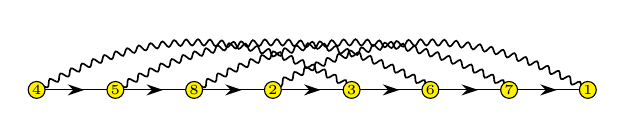
\begin{tikzpicture}
    \def \R {0.8}
    \def \ratio {0.5}
    \tikzstyle{every node}=[draw, fill=yellow, circle,inner sep=.5pt,font=\tiny];
    \begin{scope}[yshift= -\R cm, scale=1, xscale = -1]
    \coordinate (a8) at (-2.5000, 0);
    \coordinate (a7) at (-1.5000, 0);
    \coordinate (a6) at (-0.5000, 0);
    \coordinate (a5) at (0.5000, 0);
    \coordinate (a4) at (1.5000, 0);
    \coordinate (a3) at (2.5000, 0);
    \coordinate (a2) at (3.5000, 0);
    \coordinate (a1) at (-3.5000, 0);
    \draw[bareG] (a8) -- (a1);
    \draw[bareU] (a1) to [bend left] (a5);
    \draw[bareG] (a2) -- (a3);
    \draw[bareU] (a2) to [bend right] (a6);
    \draw[bareG] (a3) -- (a4);
    \draw[bareU] (a3) to [bend right] (a7);
    \draw[bareG] (a4) -- (a5);
    \draw[bareU] (a4) to [bend right] (a8);
    \draw[bareG] (a5) -- (a6);
    \draw[bareG] (a6) -- (a7);
    \draw[bareG] (a7) -- (a8);
    \end{scope}
    \node at (a1){$1$};
    \node at (a2){$4$};
    \node at (a3){$5$};
    \node at (a4){$8$};
    \node at (a5){$2$};
    \node at (a6){$3$};
    \node at (a7){$6$};
    \node at (a8){$7$};
    \end{tikzpicture}
    &
    
    
    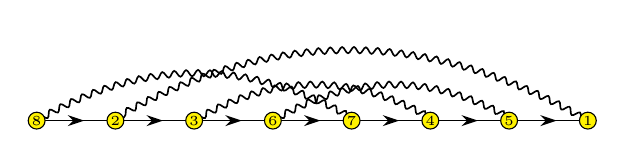
\begin{tikzpicture}
    \def \R {0.8}
    \def \ratio {0.5}
    \tikzstyle{every node}=[draw, fill=yellow, circle,inner sep=.5pt,font=\tiny];
    \begin{scope}[yshift= -\R cm, scale=1, xscale = -1]
    \coordinate (a8) at (-2.5000, 0);
    \coordinate (a7) at (-1.5000, 0);
    \coordinate (a6) at (-0.5000, 0);
    \coordinate (a5) at (0.5000, 0);
    \coordinate (a4) at (1.5000, 0);
    \coordinate (a3) at (2.5000, 0);
    \coordinate (a2) at (3.5000, 0);
    \coordinate (a1) at (-3.5000, 0);
    \draw[bareG] (a8) -- (a1);
    \draw[bareU] (a1) to [bend left] (a3);
    \draw[bareG] (a2) -- (a3);
    \draw[bareU] (a2) to [bend right] (a6);
    \draw[bareG] (a3) -- (a4);
    \draw[bareG] (a4) -- (a5);
    \draw[bareU] (a4) to [bend right] (a7);
    \draw[bareG] (a5) -- (a6);
    \draw[bareU] (a5) to [bend right] (a8);
    \draw[bareG] (a6) -- (a7);
    \draw[bareG] (a7) -- (a8);
    \end{scope}
    \node at (a1){$1$};
    \node at (a2){$8$};
    \node at (a3){$2$};
    \node at (a4){$3$};
    \node at (a5){$6$};
    \node at (a6){$7$};
    \node at (a7){$4$};
    \node at (a8){$5$};
    \end{tikzpicture}
    &
    
    
    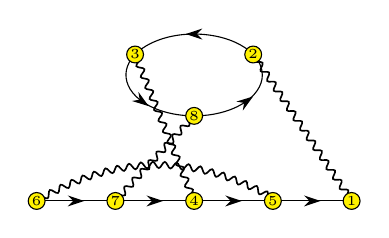
\begin{tikzpicture}
    \def \R {0.8}
    \def \ratio {0.5}
    \tikzstyle{every node}=[draw, fill=yellow, circle,inner sep=.5pt,font=\tiny];
    \begin{scope}[yshift= -\R cm, scale=1, xscale = -1]
    \coordinate (a5) at (-1.0000, 0);
    \coordinate (a4) at (0.0000, 0);
    \coordinate (a3) at (1.0000, 0);
    \coordinate (a2) at (2.0000, 0);
    \coordinate (a1) at (-2.0000, 0);
    \draw[bareG] (a5) -- (a1);
    \draw[bareG] (a2) -- (a3);
    \draw[bareU] (a2) to [bend right] (a5);
    \draw[bareG] (a3) -- (a4);
    \draw[bareG] (a4) -- (a5);
    \end{scope}
    \begin{scope}[xshift=0.0000*\R cm, yshift =1.0000*\R cm, yscale=0.6]
    \def \n {3}
    \def \r {1.7321*\ratio cm}
    \def \twist {30}
    \foreach \s in {1,...,\n}{
    \draw[bareG] ({360/\n * (\s - 1)+\twist}:\r) arc ({360/\n * (\s - 1)+\twist}:{360/\n * (\s)+\twist}:\r);}
    \coordinate (b1) at ({360/\n *(0)+\twist}:\r);
    \coordinate (b2) at ({360/\n *(1)+\twist}:\r);
    \coordinate (b3) at ({360/\n *(2)+\twist}:\r);
    \end{scope}
    \draw[bareU] (a1) -- (b1);
    \draw[bareU] (a3) -- (b3);
    \draw[bareU] (a4) -- (b2);
    \node at (a1){$1$};
    \node at (a2){$6$};
    \node at (a3){$7$};
    \node at (a4){$4$};
    \node at (a5){$5$};
    \node at (b1){$2$};
    \node at (b2){$3$};
    \node at (b3){$8$};
    \end{tikzpicture}
    &
    
    
    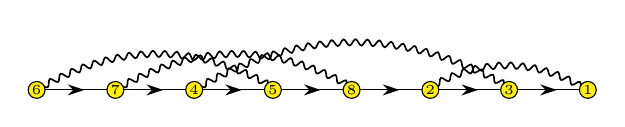
\begin{tikzpicture}
    \def \R {0.8}
    \def \ratio {0.5}
    \tikzstyle{every node}=[draw, fill=yellow, circle,inner sep=.5pt,font=\tiny];
    \begin{scope}[yshift= -\R cm, scale=1, xscale = -1]
    \coordinate (a8) at (-2.5000, 0);
    \coordinate (a7) at (-1.5000, 0);
    \coordinate (a6) at (-0.5000, 0);
    \coordinate (a5) at (0.5000, 0);
    \coordinate (a4) at (1.5000, 0);
    \coordinate (a3) at (2.5000, 0);
    \coordinate (a2) at (3.5000, 0);
    \coordinate (a1) at (-3.5000, 0);
    \draw[bareG] (a8) -- (a1);
    \draw[bareU] (a1) to [bend left] (a7);
    \draw[bareG] (a2) -- (a3);
    \draw[bareU] (a2) to [bend right] (a5);
    \draw[bareG] (a3) -- (a4);
    \draw[bareU] (a3) to [bend right] (a6);
    \draw[bareG] (a4) -- (a5);
    \draw[bareU] (a4) to [bend right] (a8);
    \draw[bareG] (a5) -- (a6);
    \draw[bareG] (a6) -- (a7);
    \draw[bareG] (a7) -- (a8);
    \end{scope}
    \node at (a1){$1$};
    \node at (a2){$6$};
    \node at (a3){$7$};
    \node at (a4){$4$};
    \node at (a5){$5$};
    \node at (a6){$8$};
    \node at (a7){$2$};
    \node at (a8){$3$};
    \end{tikzpicture}
    &
    
    
    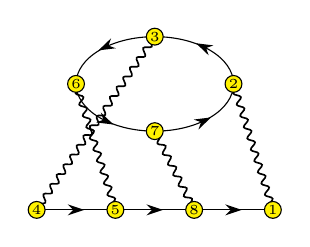
\begin{tikzpicture}
    \def \R {0.8}
    \def \ratio {0.5}
    \tikzstyle{every node}=[draw, fill=yellow, circle,inner sep=.5pt,font=\tiny];
    \begin{scope}[yshift= -\R cm, scale=1, xscale = -1]
    \coordinate (a4) at (-0.5000, 0);
    \coordinate (a3) at (0.5000, 0);
    \coordinate (a2) at (1.5000, 0);
    \coordinate (a1) at (-1.5000, 0);
    \draw[bareG] (a4) -- (a1);
    \draw[bareG] (a2) -- (a3);
    \draw[bareG] (a3) -- (a4);
    \end{scope}
    \begin{scope}[xshift=0.0000*\R cm, yshift =1.0000*\R cm, yscale=0.6]
    \def \n {4}
    \def \r {2.0000*\ratio cm}
    \def \twist {0}
    \foreach \s in {1,...,\n}{
    \draw[bareG] ({360/\n * (\s - 1)+\twist}:\r) arc ({360/\n * (\s - 1)+\twist}:{360/\n * (\s)+\twist}:\r);}
    \coordinate (b1) at ({360/\n *(0)+\twist}:\r);
    \coordinate (b2) at ({360/\n *(1)+\twist}:\r);
    \coordinate (b3) at ({360/\n *(2)+\twist}:\r);
    \coordinate (b4) at ({360/\n *(3)+\twist}:\r);
    \end{scope}
    \draw[bareU] (a1) -- (b1);
    \draw[bareU] (a2) -- (b2);
    \draw[bareU] (a3) -- (b3);
    \draw[bareU] (a4) -- (b4);
    \node at (a1){$1$};
    \node at (a2){$4$};
    \node at (a3){$5$};
    \node at (a4){$8$};
    \node at (b1){$2$};
    \node at (b2){$3$};
    \node at (b3){$6$};
    \node at (b4){$7$};
    \end{tikzpicture}
    &
    
    
    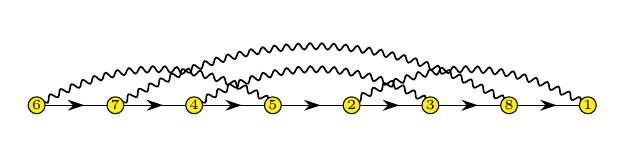
\begin{tikzpicture}
    \def \R {0.8}
    \def \ratio {0.5}
    \tikzstyle{every node}=[draw, fill=yellow, circle,inner sep=.5pt,font=\tiny];
    \begin{scope}[yshift= -\R cm, scale=1, xscale = -1]
    \coordinate (a8) at (-2.5000, 0);
    \coordinate (a7) at (-1.5000, 0);
    \coordinate (a6) at (-0.5000, 0);
    \coordinate (a5) at (0.5000, 0);
    \coordinate (a4) at (1.5000, 0);
    \coordinate (a3) at (2.5000, 0);
    \coordinate (a2) at (3.5000, 0);
    \coordinate (a1) at (-3.5000, 0);
    \draw[bareG] (a8) -- (a1);
    \draw[bareU] (a1) to [bend left] (a6);
    \draw[bareG] (a2) -- (a3);
    \draw[bareU] (a2) to [bend right] (a5);
    \draw[bareG] (a3) -- (a4);
    \draw[bareU] (a3) to [bend right] (a8);
    \draw[bareG] (a4) -- (a5);
    \draw[bareU] (a4) to [bend right] (a7);
    \draw[bareG] (a5) -- (a6);
    \draw[bareG] (a6) -- (a7);
    \draw[bareG] (a7) -- (a8);
    \end{scope}
    \node at (a1){$1$};
    \node at (a2){$6$};
    \node at (a3){$7$};
    \node at (a4){$4$};
    \node at (a5){$5$};
    \node at (a6){$2$};
    \node at (a7){$3$};
    \node at (a8){$8$};
    \end{tikzpicture}
    &
    
    
    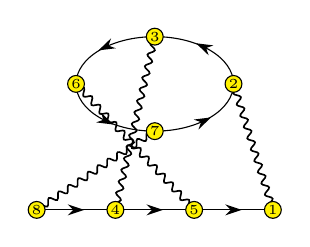
\begin{tikzpicture}
    \def \R {0.8}
    \def \ratio {0.5}
    \tikzstyle{every node}=[draw, fill=yellow, circle,inner sep=.5pt,font=\tiny];
    \begin{scope}[yshift= -\R cm, scale=1, xscale = -1]
    \coordinate (a4) at (-0.5000, 0);
    \coordinate (a3) at (0.5000, 0);
    \coordinate (a2) at (1.5000, 0);
    \coordinate (a1) at (-1.5000, 0);
    \draw[bareG] (a4) -- (a1);
    \draw[bareG] (a2) -- (a3);
    \draw[bareG] (a3) -- (a4);
    \end{scope}
    \begin{scope}[xshift=0.0000*\R cm, yshift =1.0000*\R cm, yscale=0.6]
    \def \n {4}
    \def \r {2.0000*\ratio cm}
    \def \twist {0}
    \foreach \s in {1,...,\n}{
    \draw[bareG] ({360/\n * (\s - 1)+\twist}:\r) arc ({360/\n * (\s - 1)+\twist}:{360/\n * (\s)+\twist}:\r);}
    \coordinate (b1) at ({360/\n *(0)+\twist}:\r);
    \coordinate (b2) at ({360/\n *(1)+\twist}:\r);
    \coordinate (b3) at ({360/\n *(2)+\twist}:\r);
    \coordinate (b4) at ({360/\n *(3)+\twist}:\r);
    \end{scope}
    \draw[bareU] (a1) -- (b1);
    \draw[bareU] (a2) -- (b4);
    \draw[bareU] (a3) -- (b2);
    \draw[bareU] (a4) -- (b3);
    \node at (a1){$1$};
    \node at (a2){$8$};
    \node at (a3){$4$};
    \node at (a4){$5$};
    \node at (b1){$2$};
    \node at (b2){$3$};
    \node at (b3){$6$};
    \node at (b4){$7$};
    \end{tikzpicture}
    &
    
    
    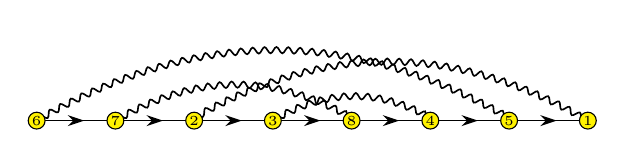
\begin{tikzpicture}
    \def \R {0.8}
    \def \ratio {0.5}
    \tikzstyle{every node}=[draw, fill=yellow, circle,inner sep=.5pt,font=\tiny];
    \begin{scope}[yshift= -\R cm, scale=1, xscale = -1]
    \coordinate (a8) at (-2.5000, 0);
    \coordinate (a7) at (-1.5000, 0);
    \coordinate (a6) at (-0.5000, 0);
    \coordinate (a5) at (0.5000, 0);
    \coordinate (a4) at (1.5000, 0);
    \coordinate (a3) at (2.5000, 0);
    \coordinate (a2) at (3.5000, 0);
    \coordinate (a1) at (-3.5000, 0);
    \draw[bareG] (a8) -- (a1);
    \draw[bareU] (a1) to [bend left] (a4);
    \draw[bareG] (a2) -- (a3);
    \draw[bareU] (a2) to [bend right] (a8);
    \draw[bareG] (a3) -- (a4);
    \draw[bareU] (a3) to [bend right] (a6);
    \draw[bareG] (a4) -- (a5);
    \draw[bareG] (a5) -- (a6);
    \draw[bareU] (a5) to [bend right] (a7);
    \draw[bareG] (a6) -- (a7);
    \draw[bareG] (a7) -- (a8);
    \end{scope}
    \node at (a1){$1$};
    \node at (a2){$6$};
    \node at (a3){$7$};
    \node at (a4){$2$};
    \node at (a5){$3$};
    \node at (a6){$8$};
    \node at (a7){$4$};
    \node at (a8){$5$};
    \end{tikzpicture}
    &
    
    
    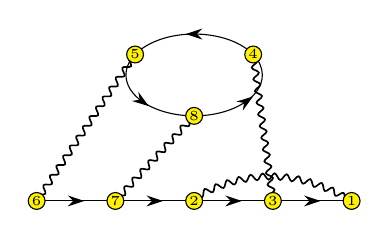
\begin{tikzpicture}
    \def \R {0.8}
    \def \ratio {0.5}
    \tikzstyle{every node}=[draw, fill=yellow, circle,inner sep=.5pt,font=\tiny];
    \begin{scope}[yshift= -\R cm, scale=1, xscale = -1]
    \coordinate (a5) at (-1.0000, 0);
    \coordinate (a4) at (0.0000, 0);
    \coordinate (a3) at (1.0000, 0);
    \coordinate (a2) at (2.0000, 0);
    \coordinate (a1) at (-2.0000, 0);
    \draw[bareG] (a5) -- (a1);
    \draw[bareU] (a1) to [bend left] (a4);
    \draw[bareG] (a2) -- (a3);
    \draw[bareG] (a3) -- (a4);
    \draw[bareG] (a4) -- (a5);
    \end{scope}
    \begin{scope}[xshift=0.0000*\R cm, yshift =1.0000*\R cm, yscale=0.6]
    \def \n {3}
    \def \r {1.7321*\ratio cm}
    \def \twist {30}
    \foreach \s in {1,...,\n}{
    \draw[bareG] ({360/\n * (\s - 1)+\twist}:\r) arc ({360/\n * (\s - 1)+\twist}:{360/\n * (\s)+\twist}:\r);}
    \coordinate (b1) at ({360/\n *(0)+\twist}:\r);
    \coordinate (b2) at ({360/\n *(1)+\twist}:\r);
    \coordinate (b3) at ({360/\n *(2)+\twist}:\r);
    \end{scope}
    \draw[bareU] (a2) -- (b2);
    \draw[bareU] (a3) -- (b3);
    \draw[bareU] (a5) -- (b1);
    \node at (a1){$1$};
    \node at (a2){$6$};
    \node at (a3){$7$};
    \node at (a4){$2$};
    \node at (a5){$3$};
    \node at (b1){$4$};
    \node at (b2){$5$};
    \node at (b3){$8$};
    \end{tikzpicture}
    &
    
    
    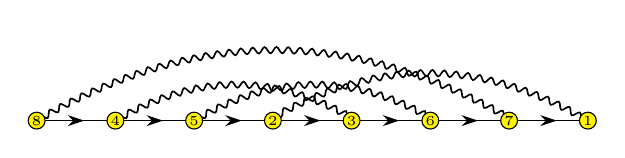
\begin{tikzpicture}
    \def \R {0.8}
    \def \ratio {0.5}
    \tikzstyle{every node}=[draw, fill=yellow, circle,inner sep=.5pt,font=\tiny];
    \begin{scope}[yshift= -\R cm, scale=1, xscale = -1]
    \coordinate (a8) at (-2.5000, 0);
    \coordinate (a7) at (-1.5000, 0);
    \coordinate (a6) at (-0.5000, 0);
    \coordinate (a5) at (0.5000, 0);
    \coordinate (a4) at (1.5000, 0);
    \coordinate (a3) at (2.5000, 0);
    \coordinate (a2) at (3.5000, 0);
    \coordinate (a1) at (-3.5000, 0);
    \draw[bareG] (a8) -- (a1);
    \draw[bareU] (a1) to [bend left] (a5);
    \draw[bareG] (a2) -- (a3);
    \draw[bareU] (a2) to [bend right] (a8);
    \draw[bareG] (a3) -- (a4);
    \draw[bareU] (a3) to [bend right] (a6);
    \draw[bareG] (a4) -- (a5);
    \draw[bareU] (a4) to [bend right] (a7);
    \draw[bareG] (a5) -- (a6);
    \draw[bareG] (a6) -- (a7);
    \draw[bareG] (a7) -- (a8);
    \end{scope}
    \node at (a1){$1$};
    \node at (a2){$8$};
    \node at (a3){$4$};
    \node at (a4){$5$};
    \node at (a5){$2$};
    \node at (a6){$3$};
    \node at (a7){$6$};
    \node at (a8){$7$};
    \end{tikzpicture}
    &
    
    
    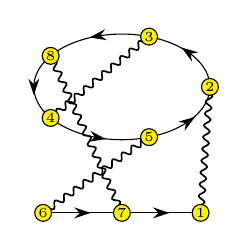
\begin{tikzpicture}
    \def \R {0.8}
    \def \ratio {0.5}
    \tikzstyle{every node}=[draw, fill=yellow, circle,inner sep=.5pt,font=\tiny];
    \begin{scope}[yshift= -\R cm, scale=1, xscale = -1]
    \coordinate (a3) at (0.0000, 0);
    \coordinate (a2) at (1.0000, 0);
    \coordinate (a1) at (-1.0000, 0);
    \draw[bareG] (a3) -- (a1);
    \draw[bareG] (a2) -- (a3);
    \end{scope}
    \begin{scope}[xshift=0.0000*\R cm, yshift =1.0000*\R cm, yscale=0.6]
    \def \n {5}
    \def \r {2.2361*\ratio cm}
    \def \twist {0}
    \foreach \s in {1,...,\n}{
    \draw[bareG] ({360/\n * (\s - 1)+\twist}:\r) arc ({360/\n * (\s - 1)+\twist}:{360/\n * (\s)+\twist}:\r);}
    \coordinate (b1) at ({360/\n *(0)+\twist}:\r);
    \coordinate (b2) at ({360/\n *(1)+\twist}:\r);
    \coordinate (b3) at ({360/\n *(2)+\twist}:\r);
    \coordinate (b4) at ({360/\n *(3)+\twist}:\r);
    \coordinate (b5) at ({360/\n *(4)+\twist}:\r);
    \end{scope}
    \draw[bareU] (a1) -- (b1);
    \draw[bareU] (a2) -- (b5);
    \draw[bareU] (a3) -- (b3);
    \draw[bareU] (b2) -- (b4);
    \node at (a1){$1$};
    \node at (a2){$6$};
    \node at (a3){$7$};
    \node at (b1){$2$};
    \node at (b2){$3$};
    \node at (b3){$8$};
    \node at (b4){$4$};
    \node at (b5){$5$};
    \end{tikzpicture}
    &
    
    
    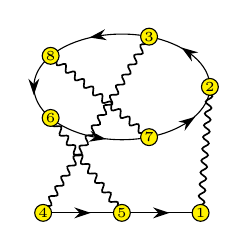
\begin{tikzpicture}
    \def \R {0.8}
    \def \ratio {0.5}
    \tikzstyle{every node}=[draw, fill=yellow, circle,inner sep=.5pt,font=\tiny];
    \begin{scope}[yshift= -\R cm, scale=1, xscale = -1]
    \coordinate (a3) at (0.0000, 0);
    \coordinate (a2) at (1.0000, 0);
    \coordinate (a1) at (-1.0000, 0);
    \draw[bareG] (a3) -- (a1);
    \draw[bareG] (a2) -- (a3);
    \end{scope}
    \begin{scope}[xshift=0.0000*\R cm, yshift =1.0000*\R cm, yscale=0.6]
    \def \n {5}
    \def \r {2.2361*\ratio cm}
    \def \twist {0}
    \foreach \s in {1,...,\n}{
    \draw[bareG] ({360/\n * (\s - 1)+\twist}:\r) arc ({360/\n * (\s - 1)+\twist}:{360/\n * (\s)+\twist}:\r);}
    \coordinate (b1) at ({360/\n *(0)+\twist}:\r);
    \coordinate (b2) at ({360/\n *(1)+\twist}:\r);
    \coordinate (b3) at ({360/\n *(2)+\twist}:\r);
    \coordinate (b4) at ({360/\n *(3)+\twist}:\r);
    \coordinate (b5) at ({360/\n *(4)+\twist}:\r);
    \end{scope}
    \draw[bareU] (a1) -- (b1);
    \draw[bareU] (a2) -- (b2);
    \draw[bareU] (a3) -- (b4);
    \draw[bareU] (b3) -- (b5);
    \node at (a1){$1$};
    \node at (a2){$4$};
    \node at (a3){$5$};
    \node at (b1){$2$};
    \node at (b2){$3$};
    \node at (b3){$8$};
    \node at (b4){$6$};
    \node at (b5){$7$};
    \end{tikzpicture}
    &
    
    
    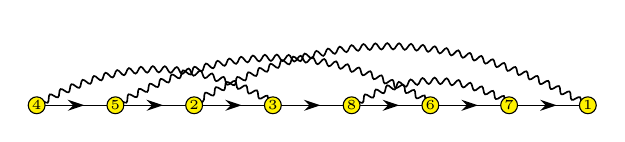
\begin{tikzpicture}
    \def \R {0.8}
    \def \ratio {0.5}
    \tikzstyle{every node}=[draw, fill=yellow, circle,inner sep=.5pt,font=\tiny];
    \begin{scope}[yshift= -\R cm, scale=1, xscale = -1]
    \coordinate (a8) at (-2.5000, 0);
    \coordinate (a7) at (-1.5000, 0);
    \coordinate (a6) at (-0.5000, 0);
    \coordinate (a5) at (0.5000, 0);
    \coordinate (a4) at (1.5000, 0);
    \coordinate (a3) at (2.5000, 0);
    \coordinate (a2) at (3.5000, 0);
    \coordinate (a1) at (-3.5000, 0);
    \draw[bareG] (a8) -- (a1);
    \draw[bareU] (a1) to [bend left] (a4);
    \draw[bareG] (a2) -- (a3);
    \draw[bareU] (a2) to [bend right] (a5);
    \draw[bareG] (a3) -- (a4);
    \draw[bareU] (a3) to [bend right] (a7);
    \draw[bareG] (a4) -- (a5);
    \draw[bareG] (a5) -- (a6);
    \draw[bareG] (a6) -- (a7);
    \draw[bareU] (a6) to [bend right] (a8);
    \draw[bareG] (a7) -- (a8);
    \end{scope}
    \node at (a1){$1$};
    \node at (a2){$4$};
    \node at (a3){$5$};
    \node at (a4){$2$};
    \node at (a5){$3$};
    \node at (a6){$8$};
    \node at (a7){$6$};
    \node at (a8){$7$};
    \end{tikzpicture}
    &
    
    
    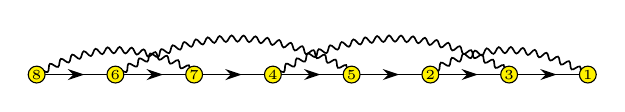
\begin{tikzpicture}
    \def \R {0.8}
    \def \ratio {0.5}
    \tikzstyle{every node}=[draw, fill=yellow, circle,inner sep=.5pt,font=\tiny];
    \begin{scope}[yshift= -\R cm, scale=1, xscale = -1]
    \coordinate (a8) at (-2.5000, 0);
    \coordinate (a7) at (-1.5000, 0);
    \coordinate (a6) at (-0.5000, 0);
    \coordinate (a5) at (0.5000, 0);
    \coordinate (a4) at (1.5000, 0);
    \coordinate (a3) at (2.5000, 0);
    \coordinate (a2) at (3.5000, 0);
    \coordinate (a1) at (-3.5000, 0);
    \draw[bareG] (a8) -- (a1);
    \draw[bareU] (a1) to [bend left] (a7);
    \draw[bareG] (a2) -- (a3);
    \draw[bareU] (a2) to [bend right] (a4);
    \draw[bareG] (a3) -- (a4);
    \draw[bareU] (a3) to [bend right] (a6);
    \draw[bareG] (a4) -- (a5);
    \draw[bareG] (a5) -- (a6);
    \draw[bareU] (a5) to [bend right] (a8);
    \draw[bareG] (a6) -- (a7);
    \draw[bareG] (a7) -- (a8);
    \end{scope}
    \node at (a1){$1$};
    \node at (a2){$8$};
    \node at (a3){$6$};
    \node at (a4){$7$};
    \node at (a5){$4$};
    \node at (a6){$5$};
    \node at (a7){$2$};
    \node at (a8){$3$};
    \end{tikzpicture}
    &
    
    
    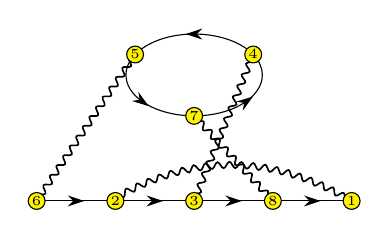
\begin{tikzpicture}
    \def \R {0.8}
    \def \ratio {0.5}
    \tikzstyle{every node}=[draw, fill=yellow, circle,inner sep=.5pt,font=\tiny];
    \begin{scope}[yshift= -\R cm, scale=1, xscale = -1]
    \coordinate (a5) at (-1.0000, 0);
    \coordinate (a4) at (0.0000, 0);
    \coordinate (a3) at (1.0000, 0);
    \coordinate (a2) at (2.0000, 0);
    \coordinate (a1) at (-2.0000, 0);
    \draw[bareG] (a5) -- (a1);
    \draw[bareU] (a1) to [bend left] (a3);
    \draw[bareG] (a2) -- (a3);
    \draw[bareG] (a3) -- (a4);
    \draw[bareG] (a4) -- (a5);
    \end{scope}
    \begin{scope}[xshift=0.0000*\R cm, yshift =1.0000*\R cm, yscale=0.6]
    \def \n {3}
    \def \r {1.7321*\ratio cm}
    \def \twist {30}
    \foreach \s in {1,...,\n}{
    \draw[bareG] ({360/\n * (\s - 1)+\twist}:\r) arc ({360/\n * (\s - 1)+\twist}:{360/\n * (\s)+\twist}:\r);}
    \coordinate (b1) at ({360/\n *(0)+\twist}:\r);
    \coordinate (b2) at ({360/\n *(1)+\twist}:\r);
    \coordinate (b3) at ({360/\n *(2)+\twist}:\r);
    \end{scope}
    \draw[bareU] (a2) -- (b2);
    \draw[bareU] (a4) -- (b1);
    \draw[bareU] (a5) -- (b3);
    \node at (a1){$1$};
    \node at (a2){$6$};
    \node at (a3){$2$};
    \node at (a4){$3$};
    \node at (a5){$8$};
    \node at (b1){$4$};
    \node at (b2){$5$};
    \node at (b3){$7$};
    \end{tikzpicture}
    &
    
    
    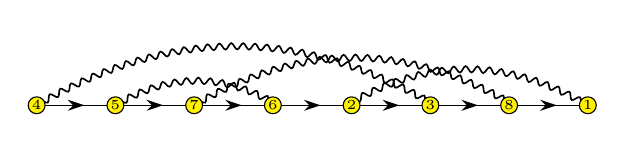
\begin{tikzpicture}
    \def \R {0.8}
    \def \ratio {0.5}
    \tikzstyle{every node}=[draw, fill=yellow, circle,inner sep=.5pt,font=\tiny];
    \begin{scope}[yshift= -\R cm, scale=1, xscale = -1]
    \coordinate (a8) at (-2.5000, 0);
    \coordinate (a7) at (-1.5000, 0);
    \coordinate (a6) at (-0.5000, 0);
    \coordinate (a5) at (0.5000, 0);
    \coordinate (a4) at (1.5000, 0);
    \coordinate (a3) at (2.5000, 0);
    \coordinate (a2) at (3.5000, 0);
    \coordinate (a1) at (-3.5000, 0);
    \draw[bareG] (a8) -- (a1);
    \draw[bareU] (a1) to [bend left] (a6);
    \draw[bareG] (a2) -- (a3);
    \draw[bareU] (a2) to [bend right] (a7);
    \draw[bareG] (a3) -- (a4);
    \draw[bareU] (a3) to [bend right] (a5);
    \draw[bareG] (a4) -- (a5);
    \draw[bareU] (a4) to [bend right] (a8);
    \draw[bareG] (a5) -- (a6);
    \draw[bareG] (a6) -- (a7);
    \draw[bareG] (a7) -- (a8);
    \end{scope}
    \node at (a1){$1$};
    \node at (a2){$4$};
    \node at (a3){$5$};
    \node at (a4){$7$};
    \node at (a5){$6$};
    \node at (a6){$2$};
    \node at (a7){$3$};
    \node at (a8){$8$};
    \end{tikzpicture}
    &
    
    
    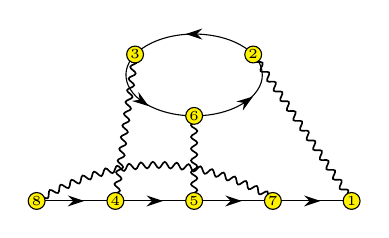
\begin{tikzpicture}
    \def \R {0.8}
    \def \ratio {0.5}
    \tikzstyle{every node}=[draw, fill=yellow, circle,inner sep=.5pt,font=\tiny];
    \begin{scope}[yshift= -\R cm, scale=1, xscale = -1]
    \coordinate (a5) at (-1.0000, 0);
    \coordinate (a4) at (0.0000, 0);
    \coordinate (a3) at (1.0000, 0);
    \coordinate (a2) at (2.0000, 0);
    \coordinate (a1) at (-2.0000, 0);
    \draw[bareG] (a5) -- (a1);
    \draw[bareG] (a2) -- (a3);
    \draw[bareU] (a2) to [bend right] (a5);
    \draw[bareG] (a3) -- (a4);
    \draw[bareG] (a4) -- (a5);
    \end{scope}
    \begin{scope}[xshift=0.0000*\R cm, yshift =1.0000*\R cm, yscale=0.6]
    \def \n {3}
    \def \r {1.7321*\ratio cm}
    \def \twist {30}
    \foreach \s in {1,...,\n}{
    \draw[bareG] ({360/\n * (\s - 1)+\twist}:\r) arc ({360/\n * (\s - 1)+\twist}:{360/\n * (\s)+\twist}:\r);}
    \coordinate (b1) at ({360/\n *(0)+\twist}:\r);
    \coordinate (b2) at ({360/\n *(1)+\twist}:\r);
    \coordinate (b3) at ({360/\n *(2)+\twist}:\r);
    \end{scope}
    \draw[bareU] (a1) -- (b1);
    \draw[bareU] (a3) -- (b2);
    \draw[bareU] (a4) -- (b3);
    \node at (a1){$1$};
    \node at (a2){$8$};
    \node at (a3){$4$};
    \node at (a4){$5$};
    \node at (a5){$7$};
    \node at (b1){$2$};
    \node at (b2){$3$};
    \node at (b3){$6$};
    \end{tikzpicture}
    &
    
    
    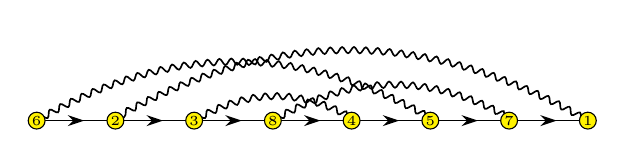
\begin{tikzpicture}
    \def \R {0.8}
    \def \ratio {0.5}
    \tikzstyle{every node}=[draw, fill=yellow, circle,inner sep=.5pt,font=\tiny];
    \begin{scope}[yshift= -\R cm, scale=1, xscale = -1]
    \coordinate (a8) at (-2.5000, 0);
    \coordinate (a7) at (-1.5000, 0);
    \coordinate (a6) at (-0.5000, 0);
    \coordinate (a5) at (0.5000, 0);
    \coordinate (a4) at (1.5000, 0);
    \coordinate (a3) at (2.5000, 0);
    \coordinate (a2) at (3.5000, 0);
    \coordinate (a1) at (-3.5000, 0);
    \draw[bareG] (a8) -- (a1);
    \draw[bareU] (a1) to [bend left] (a3);
    \draw[bareG] (a2) -- (a3);
    \draw[bareU] (a2) to [bend right] (a7);
    \draw[bareG] (a3) -- (a4);
    \draw[bareG] (a4) -- (a5);
    \draw[bareU] (a4) to [bend right] (a6);
    \draw[bareG] (a5) -- (a6);
    \draw[bareU] (a5) to [bend right] (a8);
    \draw[bareG] (a6) -- (a7);
    \draw[bareG] (a7) -- (a8);
    \end{scope}
    \node at (a1){$1$};
    \node at (a2){$6$};
    \node at (a3){$2$};
    \node at (a4){$3$};
    \node at (a5){$8$};
    \node at (a6){$4$};
    \node at (a7){$5$};
    \node at (a8){$7$};
    \end{tikzpicture}
    &
    
    
    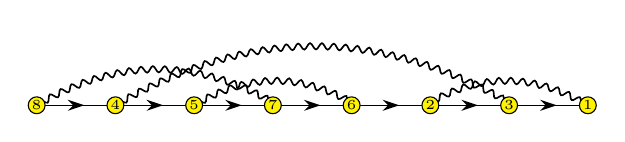
\begin{tikzpicture}
    \def \R {0.8}
    \def \ratio {0.5}
    \tikzstyle{every node}=[draw, fill=yellow, circle,inner sep=.5pt,font=\tiny];
    \begin{scope}[yshift= -\R cm, scale=1, xscale = -1]
    \coordinate (a8) at (-2.5000, 0);
    \coordinate (a7) at (-1.5000, 0);
    \coordinate (a6) at (-0.5000, 0);
    \coordinate (a5) at (0.5000, 0);
    \coordinate (a4) at (1.5000, 0);
    \coordinate (a3) at (2.5000, 0);
    \coordinate (a2) at (3.5000, 0);
    \coordinate (a1) at (-3.5000, 0);
    \draw[bareG] (a8) -- (a1);
    \draw[bareU] (a1) to [bend left] (a7);
    \draw[bareG] (a2) -- (a3);
    \draw[bareU] (a2) to [bend right] (a5);
    \draw[bareG] (a3) -- (a4);
    \draw[bareU] (a3) to [bend right] (a8);
    \draw[bareG] (a4) -- (a5);
    \draw[bareU] (a4) to [bend right] (a6);
    \draw[bareG] (a5) -- (a6);
    \draw[bareG] (a6) -- (a7);
    \draw[bareG] (a7) -- (a8);
    \end{scope}
    \node at (a1){$1$};
    \node at (a2){$8$};
    \node at (a3){$4$};
    \node at (a4){$5$};
    \node at (a5){$7$};
    \node at (a6){$6$};
    \node at (a7){$2$};
    \node at (a8){$3$};
    \end{tikzpicture}
    &
    
    
    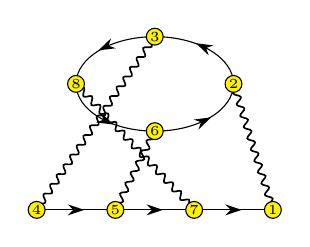
\begin{tikzpicture}
    \def \R {0.8}
    \def \ratio {0.5}
    \tikzstyle{every node}=[draw, fill=yellow, circle,inner sep=.5pt,font=\tiny];
    \begin{scope}[yshift= -\R cm, scale=1, xscale = -1]
    \coordinate (a4) at (-0.5000, 0);
    \coordinate (a3) at (0.5000, 0);
    \coordinate (a2) at (1.5000, 0);
    \coordinate (a1) at (-1.5000, 0);
    \draw[bareG] (a4) -- (a1);
    \draw[bareG] (a2) -- (a3);
    \draw[bareG] (a3) -- (a4);
    \end{scope}
    \begin{scope}[xshift=0.0000*\R cm, yshift =1.0000*\R cm, yscale=0.6]
    \def \n {4}
    \def \r {2.0000*\ratio cm}
    \def \twist {0}
    \foreach \s in {1,...,\n}{
    \draw[bareG] ({360/\n * (\s - 1)+\twist}:\r) arc ({360/\n * (\s - 1)+\twist}:{360/\n * (\s)+\twist}:\r);}
    \coordinate (b1) at ({360/\n *(0)+\twist}:\r);
    \coordinate (b2) at ({360/\n *(1)+\twist}:\r);
    \coordinate (b3) at ({360/\n *(2)+\twist}:\r);
    \coordinate (b4) at ({360/\n *(3)+\twist}:\r);
    \end{scope}
    \draw[bareU] (a1) -- (b1);
    \draw[bareU] (a2) -- (b2);
    \draw[bareU] (a3) -- (b4);
    \draw[bareU] (a4) -- (b3);
    \node at (a1){$1$};
    \node at (a2){$4$};
    \node at (a3){$5$};
    \node at (a4){$7$};
    \node at (b1){$2$};
    \node at (b2){$3$};
    \node at (b3){$8$};
    \node at (b4){$6$};
    \end{tikzpicture}
    &
    
    
    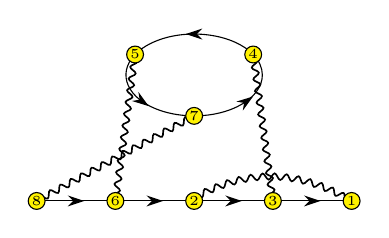
\begin{tikzpicture}
    \def \R {0.8}
    \def \ratio {0.5}
    \tikzstyle{every node}=[draw, fill=yellow, circle,inner sep=.5pt,font=\tiny];
    \begin{scope}[yshift= -\R cm, scale=1, xscale = -1]
    \coordinate (a5) at (-1.0000, 0);
    \coordinate (a4) at (0.0000, 0);
    \coordinate (a3) at (1.0000, 0);
    \coordinate (a2) at (2.0000, 0);
    \coordinate (a1) at (-2.0000, 0);
    \draw[bareG] (a5) -- (a1);
    \draw[bareU] (a1) to [bend left] (a4);
    \draw[bareG] (a2) -- (a3);
    \draw[bareG] (a3) -- (a4);
    \draw[bareG] (a4) -- (a5);
    \end{scope}
    \begin{scope}[xshift=0.0000*\R cm, yshift =1.0000*\R cm, yscale=0.6]
    \def \n {3}
    \def \r {1.7321*\ratio cm}
    \def \twist {30}
    \foreach \s in {1,...,\n}{
    \draw[bareG] ({360/\n * (\s - 1)+\twist}:\r) arc ({360/\n * (\s - 1)+\twist}:{360/\n * (\s)+\twist}:\r);}
    \coordinate (b1) at ({360/\n *(0)+\twist}:\r);
    \coordinate (b2) at ({360/\n *(1)+\twist}:\r);
    \coordinate (b3) at ({360/\n *(2)+\twist}:\r);
    \end{scope}
    \draw[bareU] (a2) -- (b3);
    \draw[bareU] (a3) -- (b2);
    \draw[bareU] (a5) -- (b1);
    \node at (a1){$1$};
    \node at (a2){$8$};
    \node at (a3){$6$};
    \node at (a4){$2$};
    \node at (a5){$3$};
    \node at (b1){$4$};
    \node at (b2){$5$};
    \node at (b3){$7$};
    \end{tikzpicture}
    &
    
    
    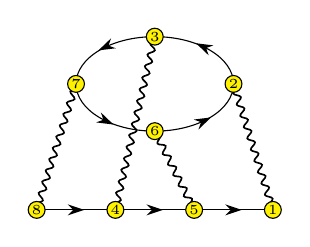
\begin{tikzpicture}
    \def \R {0.8}
    \def \ratio {0.5}
    \tikzstyle{every node}=[draw, fill=yellow, circle,inner sep=.5pt,font=\tiny];
    \begin{scope}[yshift= -\R cm, scale=1, xscale = -1]
    \coordinate (a4) at (-0.5000, 0);
    \coordinate (a3) at (0.5000, 0);
    \coordinate (a2) at (1.5000, 0);
    \coordinate (a1) at (-1.5000, 0);
    \draw[bareG] (a4) -- (a1);
    \draw[bareG] (a2) -- (a3);
    \draw[bareG] (a3) -- (a4);
    \end{scope}
    \begin{scope}[xshift=0.0000*\R cm, yshift =1.0000*\R cm, yscale=0.6]
    \def \n {4}
    \def \r {2.0000*\ratio cm}
    \def \twist {0}
    \foreach \s in {1,...,\n}{
    \draw[bareG] ({360/\n * (\s - 1)+\twist}:\r) arc ({360/\n * (\s - 1)+\twist}:{360/\n * (\s)+\twist}:\r);}
    \coordinate (b1) at ({360/\n *(0)+\twist}:\r);
    \coordinate (b2) at ({360/\n *(1)+\twist}:\r);
    \coordinate (b3) at ({360/\n *(2)+\twist}:\r);
    \coordinate (b4) at ({360/\n *(3)+\twist}:\r);
    \end{scope}
    \draw[bareU] (a1) -- (b1);
    \draw[bareU] (a2) -- (b3);
    \draw[bareU] (a3) -- (b2);
    \draw[bareU] (a4) -- (b4);
    \node at (a1){$1$};
    \node at (a2){$8$};
    \node at (a3){$4$};
    \node at (a4){$5$};
    \node at (b1){$2$};
    \node at (b2){$3$};
    \node at (b3){$7$};
    \node at (b4){$6$};
    \end{tikzpicture}
    &
    
    
    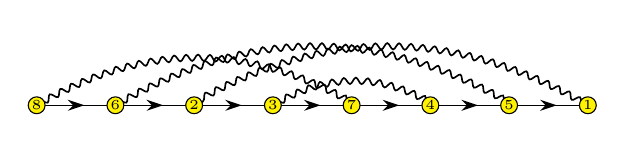
\begin{tikzpicture}
    \def \R {0.8}
    \def \ratio {0.5}
    \tikzstyle{every node}=[draw, fill=yellow, circle,inner sep=.5pt,font=\tiny];
    \begin{scope}[yshift= -\R cm, scale=1, xscale = -1]
    \coordinate (a8) at (-2.5000, 0);
    \coordinate (a7) at (-1.5000, 0);
    \coordinate (a6) at (-0.5000, 0);
    \coordinate (a5) at (0.5000, 0);
    \coordinate (a4) at (1.5000, 0);
    \coordinate (a3) at (2.5000, 0);
    \coordinate (a2) at (3.5000, 0);
    \coordinate (a1) at (-3.5000, 0);
    \draw[bareG] (a8) -- (a1);
    \draw[bareU] (a1) to [bend left] (a4);
    \draw[bareG] (a2) -- (a3);
    \draw[bareU] (a2) to [bend right] (a6);
    \draw[bareG] (a3) -- (a4);
    \draw[bareU] (a3) to [bend right] (a8);
    \draw[bareG] (a4) -- (a5);
    \draw[bareG] (a5) -- (a6);
    \draw[bareU] (a5) to [bend right] (a7);
    \draw[bareG] (a6) -- (a7);
    \draw[bareG] (a7) -- (a8);
    \end{scope}
    \node at (a1){$1$};
    \node at (a2){$8$};
    \node at (a3){$6$};
    \node at (a4){$2$};
    \node at (a5){$3$};
    \node at (a6){$7$};
    \node at (a7){$4$};
    \node at (a8){$5$};
    \end{tikzpicture}
    &
    
    
    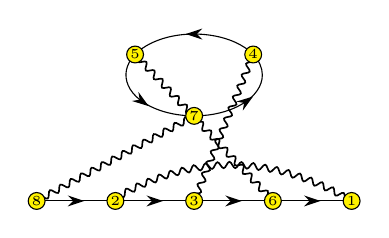
\begin{tikzpicture}
    \def \R {0.8}
    \def \ratio {0.5}
    \tikzstyle{every node}=[draw, fill=yellow, circle,inner sep=.5pt,font=\tiny];
    \begin{scope}[yshift= -\R cm, scale=1, xscale = -1]
    \coordinate (a5) at (-1.0000, 0);
    \coordinate (a4) at (0.0000, 0);
    \coordinate (a3) at (1.0000, 0);
    \coordinate (a2) at (2.0000, 0);
    \coordinate (a1) at (-2.0000, 0);
    \draw[bareG] (a5) -- (a1);
    \draw[bareU] (a1) to [bend left] (a3);
    \draw[bareG] (a2) -- (a3);
    \draw[bareG] (a3) -- (a4);
    \draw[bareG] (a4) -- (a5);
    \end{scope}
    \begin{scope}[xshift=0.0000*\R cm, yshift =1.0000*\R cm, yscale=0.6]
    \def \n {3}
    \def \r {1.7321*\ratio cm}
    \def \twist {30}
    \foreach \s in {1,...,\n}{
    \draw[bareG] ({360/\n * (\s - 1)+\twist}:\r) arc ({360/\n * (\s - 1)+\twist}:{360/\n * (\s)+\twist}:\r);}
    \coordinate (b1) at ({360/\n *(0)+\twist}:\r);
    \coordinate (b2) at ({360/\n *(1)+\twist}:\r);
    \coordinate (b3) at ({360/\n *(2)+\twist}:\r);
    \end{scope}
    \draw[bareU] (a2) -- (b3);
    \draw[bareU] (a4) -- (b1);
    \draw[bareU] (a5) -- (b2);
    \node at (a1){$1$};
    \node at (a2){$8$};
    \node at (a3){$2$};
    \node at (a4){$3$};
    \node at (a5){$6$};
    \node at (b1){$4$};
    \node at (b2){$5$};
    \node at (b3){$7$};
    \end{tikzpicture}
    &
    
    
    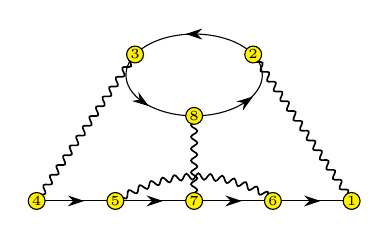
\begin{tikzpicture}
    \def \R {0.8}
    \def \ratio {0.5}
    \tikzstyle{every node}=[draw, fill=yellow, circle,inner sep=.5pt,font=\tiny];
    \begin{scope}[yshift= -\R cm, scale=1, xscale = -1]
    \coordinate (a5) at (-1.0000, 0);
    \coordinate (a4) at (0.0000, 0);
    \coordinate (a3) at (1.0000, 0);
    \coordinate (a2) at (2.0000, 0);
    \coordinate (a1) at (-2.0000, 0);
    \draw[bareG] (a5) -- (a1);
    \draw[bareG] (a2) -- (a3);
    \draw[bareG] (a3) -- (a4);
    \draw[bareU] (a3) to [bend right] (a5);
    \draw[bareG] (a4) -- (a5);
    \end{scope}
    \begin{scope}[xshift=0.0000*\R cm, yshift =1.0000*\R cm, yscale=0.6]
    \def \n {3}
    \def \r {1.7321*\ratio cm}
    \def \twist {30}
    \foreach \s in {1,...,\n}{
    \draw[bareG] ({360/\n * (\s - 1)+\twist}:\r) arc ({360/\n * (\s - 1)+\twist}:{360/\n * (\s)+\twist}:\r);}
    \coordinate (b1) at ({360/\n *(0)+\twist}:\r);
    \coordinate (b2) at ({360/\n *(1)+\twist}:\r);
    \coordinate (b3) at ({360/\n *(2)+\twist}:\r);
    \end{scope}
    \draw[bareU] (a1) -- (b1);
    \draw[bareU] (a2) -- (b2);
    \draw[bareU] (a4) -- (b3);
    \node at (a1){$1$};
    \node at (a2){$4$};
    \node at (a3){$5$};
    \node at (a4){$7$};
    \node at (a5){$6$};
    \node at (b1){$2$};
    \node at (b2){$3$};
    \node at (b3){$8$};
    \end{tikzpicture}
    &
    
    
    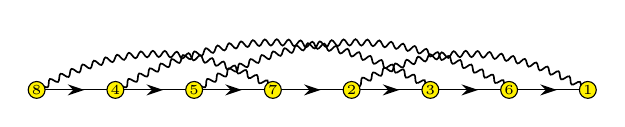
\begin{tikzpicture}
    \def \R {0.8}
    \def \ratio {0.5}
    \tikzstyle{every node}=[draw, fill=yellow, circle,inner sep=.5pt,font=\tiny];
    \begin{scope}[yshift= -\R cm, scale=1, xscale = -1]
    \coordinate (a8) at (-2.5000, 0);
    \coordinate (a7) at (-1.5000, 0);
    \coordinate (a6) at (-0.5000, 0);
    \coordinate (a5) at (0.5000, 0);
    \coordinate (a4) at (1.5000, 0);
    \coordinate (a3) at (2.5000, 0);
    \coordinate (a2) at (3.5000, 0);
    \coordinate (a1) at (-3.5000, 0);
    \draw[bareG] (a8) -- (a1);
    \draw[bareU] (a1) to [bend left] (a6);
    \draw[bareG] (a2) -- (a3);
    \draw[bareU] (a2) to [bend right] (a5);
    \draw[bareG] (a3) -- (a4);
    \draw[bareU] (a3) to [bend right] (a7);
    \draw[bareG] (a4) -- (a5);
    \draw[bareU] (a4) to [bend right] (a8);
    \draw[bareG] (a5) -- (a6);
    \draw[bareG] (a6) -- (a7);
    \draw[bareG] (a7) -- (a8);
    \end{scope}
    \node at (a1){$1$};
    \node at (a2){$8$};
    \node at (a3){$4$};
    \node at (a4){$5$};
    \node at (a5){$7$};
    \node at (a6){$2$};
    \node at (a7){$3$};
    \node at (a8){$6$};
    \end{tikzpicture}
    &
    
    
    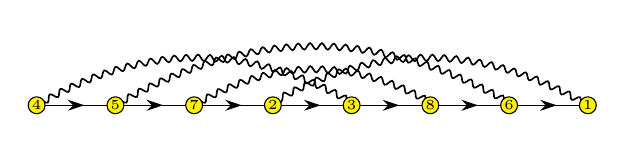
\begin{tikzpicture}
    \def \R {0.8}
    \def \ratio {0.5}
    \tikzstyle{every node}=[draw, fill=yellow, circle,inner sep=.5pt,font=\tiny];
    \begin{scope}[yshift= -\R cm, scale=1, xscale = -1]
    \coordinate (a8) at (-2.5000, 0);
    \coordinate (a7) at (-1.5000, 0);
    \coordinate (a6) at (-0.5000, 0);
    \coordinate (a5) at (0.5000, 0);
    \coordinate (a4) at (1.5000, 0);
    \coordinate (a3) at (2.5000, 0);
    \coordinate (a2) at (3.5000, 0);
    \coordinate (a1) at (-3.5000, 0);
    \draw[bareG] (a8) -- (a1);
    \draw[bareU] (a1) to [bend left] (a5);
    \draw[bareG] (a2) -- (a3);
    \draw[bareU] (a2) to [bend right] (a6);
    \draw[bareG] (a3) -- (a4);
    \draw[bareU] (a3) to [bend right] (a8);
    \draw[bareG] (a4) -- (a5);
    \draw[bareU] (a4) to [bend right] (a7);
    \draw[bareG] (a5) -- (a6);
    \draw[bareG] (a6) -- (a7);
    \draw[bareG] (a7) -- (a8);
    \end{scope}
    \node at (a1){$1$};
    \node at (a2){$4$};
    \node at (a3){$5$};
    \node at (a4){$7$};
    \node at (a5){$2$};
    \node at (a6){$3$};
    \node at (a7){$8$};
    \node at (a8){$6$};
    \end{tikzpicture}
    &
    
    
    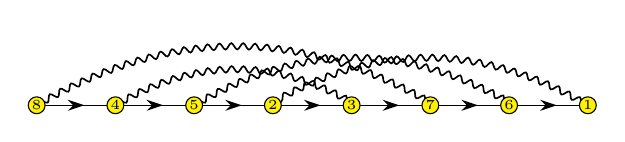
\begin{tikzpicture}
    \def \R {0.8}
    \def \ratio {0.5}
    \tikzstyle{every node}=[draw, fill=yellow, circle,inner sep=.5pt,font=\tiny];
    \begin{scope}[yshift= -\R cm, scale=1, xscale = -1]
    \coordinate (a8) at (-2.5000, 0);
    \coordinate (a7) at (-1.5000, 0);
    \coordinate (a6) at (-0.5000, 0);
    \coordinate (a5) at (0.5000, 0);
    \coordinate (a4) at (1.5000, 0);
    \coordinate (a3) at (2.5000, 0);
    \coordinate (a2) at (3.5000, 0);
    \coordinate (a1) at (-3.5000, 0);
    \draw[bareG] (a8) -- (a1);
    \draw[bareU] (a1) to [bend left] (a5);
    \draw[bareG] (a2) -- (a3);
    \draw[bareU] (a2) to [bend right] (a7);
    \draw[bareG] (a3) -- (a4);
    \draw[bareU] (a3) to [bend right] (a6);
    \draw[bareG] (a4) -- (a5);
    \draw[bareU] (a4) to [bend right] (a8);
    \draw[bareG] (a5) -- (a6);
    \draw[bareG] (a6) -- (a7);
    \draw[bareG] (a7) -- (a8);
    \end{scope}
    \node at (a1){$1$};
    \node at (a2){$8$};
    \node at (a3){$4$};
    \node at (a4){$5$};
    \node at (a5){$2$};
    \node at (a6){$3$};
    \node at (a7){$7$};
    \node at (a8){$6$};
    \end{tikzpicture}
    &
    
    
    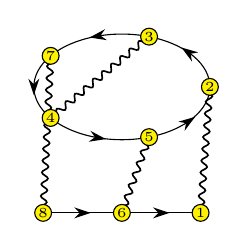
\begin{tikzpicture}
    \def \R {0.8}
    \def \ratio {0.5}
    \tikzstyle{every node}=[draw, fill=yellow, circle,inner sep=.5pt,font=\tiny];
    \begin{scope}[yshift= -\R cm, scale=1, xscale = -1]
    \coordinate (a3) at (0.0000, 0);
    \coordinate (a2) at (1.0000, 0);
    \coordinate (a1) at (-1.0000, 0);
    \draw[bareG] (a3) -- (a1);
    \draw[bareG] (a2) -- (a3);
    \end{scope}
    \begin{scope}[xshift=0.0000*\R cm, yshift =1.0000*\R cm, yscale=0.6]
    \def \n {5}
    \def \r {2.2361*\ratio cm}
    \def \twist {0}
    \foreach \s in {1,...,\n}{
    \draw[bareG] ({360/\n * (\s - 1)+\twist}:\r) arc ({360/\n * (\s - 1)+\twist}:{360/\n * (\s)+\twist}:\r);}
    \coordinate (b1) at ({360/\n *(0)+\twist}:\r);
    \coordinate (b2) at ({360/\n *(1)+\twist}:\r);
    \coordinate (b3) at ({360/\n *(2)+\twist}:\r);
    \coordinate (b4) at ({360/\n *(3)+\twist}:\r);
    \coordinate (b5) at ({360/\n *(4)+\twist}:\r);
    \end{scope}
    \draw[bareU] (a1) -- (b1);
    \draw[bareU] (a2) -- (b3);
    \draw[bareU] (a3) -- (b5);
    \draw[bareU] (b2) -- (b4);
    \node at (a1){$1$};
    \node at (a2){$8$};
    \node at (a3){$6$};
    \node at (b1){$2$};
    \node at (b2){$3$};
    \node at (b3){$7$};
    \node at (b4){$4$};
    \node at (b5){$5$};
    \end{tikzpicture}
    &
    
    
    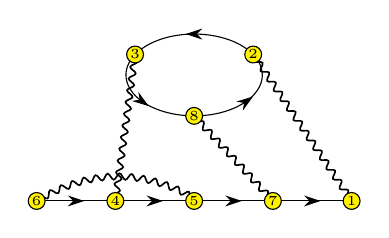
\begin{tikzpicture}
    \def \R {0.8}
    \def \ratio {0.5}
    \tikzstyle{every node}=[draw, fill=yellow, circle,inner sep=.5pt,font=\tiny];
    \begin{scope}[yshift= -\R cm, scale=1, xscale = -1]
    \coordinate (a5) at (-1.0000, 0);
    \coordinate (a4) at (0.0000, 0);
    \coordinate (a3) at (1.0000, 0);
    \coordinate (a2) at (2.0000, 0);
    \coordinate (a1) at (-2.0000, 0);
    \draw[bareG] (a5) -- (a1);
    \draw[bareG] (a2) -- (a3);
    \draw[bareU] (a2) to [bend right] (a4);
    \draw[bareG] (a3) -- (a4);
    \draw[bareG] (a4) -- (a5);
    \end{scope}
    \begin{scope}[xshift=0.0000*\R cm, yshift =1.0000*\R cm, yscale=0.6]
    \def \n {3}
    \def \r {1.7321*\ratio cm}
    \def \twist {30}
    \foreach \s in {1,...,\n}{
    \draw[bareG] ({360/\n * (\s - 1)+\twist}:\r) arc ({360/\n * (\s - 1)+\twist}:{360/\n * (\s)+\twist}:\r);}
    \coordinate (b1) at ({360/\n *(0)+\twist}:\r);
    \coordinate (b2) at ({360/\n *(1)+\twist}:\r);
    \coordinate (b3) at ({360/\n *(2)+\twist}:\r);
    \end{scope}
    \draw[bareU] (a1) -- (b1);
    \draw[bareU] (a3) -- (b2);
    \draw[bareU] (a5) -- (b3);
    \node at (a1){$1$};
    \node at (a2){$6$};
    \node at (a3){$4$};
    \node at (a4){$5$};
    \node at (a5){$7$};
    \node at (b1){$2$};
    \node at (b2){$3$};
    \node at (b3){$8$};
    \end{tikzpicture}
    &
    
    
    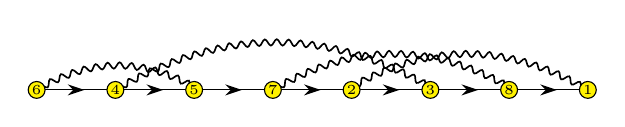
\begin{tikzpicture}
    \def \R {0.8}
    \def \ratio {0.5}
    \tikzstyle{every node}=[draw, fill=yellow, circle,inner sep=.5pt,font=\tiny];
    \begin{scope}[yshift= -\R cm, scale=1, xscale = -1]
    \coordinate (a8) at (-2.5000, 0);
    \coordinate (a7) at (-1.5000, 0);
    \coordinate (a6) at (-0.5000, 0);
    \coordinate (a5) at (0.5000, 0);
    \coordinate (a4) at (1.5000, 0);
    \coordinate (a3) at (2.5000, 0);
    \coordinate (a2) at (3.5000, 0);
    \coordinate (a1) at (-3.5000, 0);
    \draw[bareG] (a8) -- (a1);
    \draw[bareU] (a1) to [bend left] (a6);
    \draw[bareG] (a2) -- (a3);
    \draw[bareU] (a2) to [bend right] (a4);
    \draw[bareG] (a3) -- (a4);
    \draw[bareU] (a3) to [bend right] (a7);
    \draw[bareG] (a4) -- (a5);
    \draw[bareG] (a5) -- (a6);
    \draw[bareU] (a5) to [bend right] (a8);
    \draw[bareG] (a6) -- (a7);
    \draw[bareG] (a7) -- (a8);
    \end{scope}
    \node at (a1){$1$};
    \node at (a2){$6$};
    \node at (a3){$4$};
    \node at (a4){$5$};
    \node at (a5){$7$};
    \node at (a6){$2$};
    \node at (a7){$3$};
    \node at (a8){$8$};
    \end{tikzpicture}
    &
    
    
    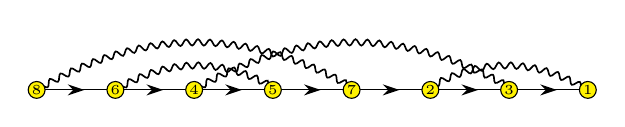
\begin{tikzpicture}
    \def \R {0.8}
    \def \ratio {0.5}
    \tikzstyle{every node}=[draw, fill=yellow, circle,inner sep=.5pt,font=\tiny];
    \begin{scope}[yshift= -\R cm, scale=1, xscale = -1]
    \coordinate (a8) at (-2.5000, 0);
    \coordinate (a7) at (-1.5000, 0);
    \coordinate (a6) at (-0.5000, 0);
    \coordinate (a5) at (0.5000, 0);
    \coordinate (a4) at (1.5000, 0);
    \coordinate (a3) at (2.5000, 0);
    \coordinate (a2) at (3.5000, 0);
    \coordinate (a1) at (-3.5000, 0);
    \draw[bareG] (a8) -- (a1);
    \draw[bareU] (a1) to [bend left] (a7);
    \draw[bareG] (a2) -- (a3);
    \draw[bareU] (a2) to [bend right] (a6);
    \draw[bareG] (a3) -- (a4);
    \draw[bareU] (a3) to [bend right] (a5);
    \draw[bareG] (a4) -- (a5);
    \draw[bareU] (a4) to [bend right] (a8);
    \draw[bareG] (a5) -- (a6);
    \draw[bareG] (a6) -- (a7);
    \draw[bareG] (a7) -- (a8);
    \end{scope}
    \node at (a1){$1$};
    \node at (a2){$8$};
    \node at (a3){$6$};
    \node at (a4){$4$};
    \node at (a5){$5$};
    \node at (a6){$7$};
    \node at (a7){$2$};
    \node at (a8){$3$};
    \end{tikzpicture}
    &
    
    
    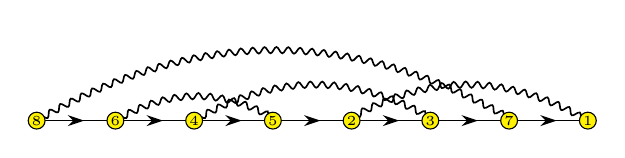
\begin{tikzpicture}
    \def \R {0.8}
    \def \ratio {0.5}
    \tikzstyle{every node}=[draw, fill=yellow, circle,inner sep=.5pt,font=\tiny];
    \begin{scope}[yshift= -\R cm, scale=1, xscale = -1]
    \coordinate (a8) at (-2.5000, 0);
    \coordinate (a7) at (-1.5000, 0);
    \coordinate (a6) at (-0.5000, 0);
    \coordinate (a5) at (0.5000, 0);
    \coordinate (a4) at (1.5000, 0);
    \coordinate (a3) at (2.5000, 0);
    \coordinate (a2) at (3.5000, 0);
    \coordinate (a1) at (-3.5000, 0);
    \draw[bareG] (a8) -- (a1);
    \draw[bareU] (a1) to [bend left] (a6);
    \draw[bareG] (a2) -- (a3);
    \draw[bareU] (a2) to [bend right] (a8);
    \draw[bareG] (a3) -- (a4);
    \draw[bareU] (a3) to [bend right] (a5);
    \draw[bareG] (a4) -- (a5);
    \draw[bareU] (a4) to [bend right] (a7);
    \draw[bareG] (a5) -- (a6);
    \draw[bareG] (a6) -- (a7);
    \draw[bareG] (a7) -- (a8);
    \end{scope}
    \node at (a1){$1$};
    \node at (a2){$8$};
    \node at (a3){$6$};
    \node at (a4){$4$};
    \node at (a5){$5$};
    \node at (a6){$2$};
    \node at (a7){$3$};
    \node at (a8){$7$};
    \end{tikzpicture}
    &
    
    
    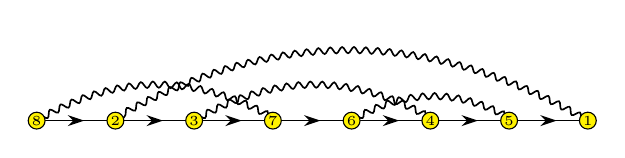
\begin{tikzpicture}
    \def \R {0.8}
    \def \ratio {0.5}
    \tikzstyle{every node}=[draw, fill=yellow, circle,inner sep=.5pt,font=\tiny];
    \begin{scope}[yshift= -\R cm, scale=1, xscale = -1]
    \coordinate (a8) at (-2.5000, 0);
    \coordinate (a7) at (-1.5000, 0);
    \coordinate (a6) at (-0.5000, 0);
    \coordinate (a5) at (0.5000, 0);
    \coordinate (a4) at (1.5000, 0);
    \coordinate (a3) at (2.5000, 0);
    \coordinate (a2) at (3.5000, 0);
    \coordinate (a1) at (-3.5000, 0);
    \draw[bareG] (a8) -- (a1);
    \draw[bareU] (a1) to [bend left] (a3);
    \draw[bareG] (a2) -- (a3);
    \draw[bareU] (a2) to [bend right] (a5);
    \draw[bareG] (a3) -- (a4);
    \draw[bareG] (a4) -- (a5);
    \draw[bareU] (a4) to [bend right] (a7);
    \draw[bareG] (a5) -- (a6);
    \draw[bareG] (a6) -- (a7);
    \draw[bareU] (a6) to [bend right] (a8);
    \draw[bareG] (a7) -- (a8);
    \end{scope}
    \node at (a1){$1$};
    \node at (a2){$8$};
    \node at (a3){$2$};
    \node at (a4){$3$};
    \node at (a5){$7$};
    \node at (a6){$6$};
    \node at (a7){$4$};
    \node at (a8){$5$};
    \end{tikzpicture}
    &
    
    
    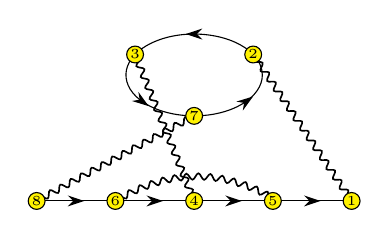
\begin{tikzpicture}
    \def \R {0.8}
    \def \ratio {0.5}
    \tikzstyle{every node}=[draw, fill=yellow, circle,inner sep=.5pt,font=\tiny];
    \begin{scope}[yshift= -\R cm, scale=1, xscale = -1]
    \coordinate (a5) at (-1.0000, 0);
    \coordinate (a4) at (0.0000, 0);
    \coordinate (a3) at (1.0000, 0);
    \coordinate (a2) at (2.0000, 0);
    \coordinate (a1) at (-2.0000, 0);
    \draw[bareG] (a5) -- (a1);
    \draw[bareG] (a2) -- (a3);
    \draw[bareG] (a3) -- (a4);
    \draw[bareU] (a3) to [bend right] (a5);
    \draw[bareG] (a4) -- (a5);
    \end{scope}
    \begin{scope}[xshift=0.0000*\R cm, yshift =1.0000*\R cm, yscale=0.6]
    \def \n {3}
    \def \r {1.7321*\ratio cm}
    \def \twist {30}
    \foreach \s in {1,...,\n}{
    \draw[bareG] ({360/\n * (\s - 1)+\twist}:\r) arc ({360/\n * (\s - 1)+\twist}:{360/\n * (\s)+\twist}:\r);}
    \coordinate (b1) at ({360/\n *(0)+\twist}:\r);
    \coordinate (b2) at ({360/\n *(1)+\twist}:\r);
    \coordinate (b3) at ({360/\n *(2)+\twist}:\r);
    \end{scope}
    \draw[bareU] (a1) -- (b1);
    \draw[bareU] (a2) -- (b3);
    \draw[bareU] (a4) -- (b2);
    \node at (a1){$1$};
    \node at (a2){$8$};
    \node at (a3){$6$};
    \node at (a4){$4$};
    \node at (a5){$5$};
    \node at (b1){$2$};
    \node at (b2){$3$};
    \node at (b3){$7$};
    \end{tikzpicture}
    &
    
    
    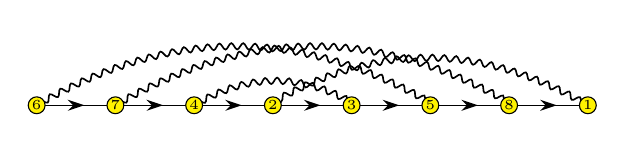
\begin{tikzpicture}
    \def \R {0.8}
    \def \ratio {0.5}
    \tikzstyle{every node}=[draw, fill=yellow, circle,inner sep=.5pt,font=\tiny];
    \begin{scope}[yshift= -\R cm, scale=1, xscale = -1]
    \coordinate (a8) at (-2.5000, 0);
    \coordinate (a7) at (-1.5000, 0);
    \coordinate (a6) at (-0.5000, 0);
    \coordinate (a5) at (0.5000, 0);
    \coordinate (a4) at (1.5000, 0);
    \coordinate (a3) at (2.5000, 0);
    \coordinate (a2) at (3.5000, 0);
    \coordinate (a1) at (-3.5000, 0);
    \draw[bareG] (a8) -- (a1);
    \draw[bareU] (a1) to [bend left] (a5);
    \draw[bareG] (a2) -- (a3);
    \draw[bareU] (a2) to [bend right] (a7);
    \draw[bareG] (a3) -- (a4);
    \draw[bareU] (a3) to [bend right] (a8);
    \draw[bareG] (a4) -- (a5);
    \draw[bareU] (a4) to [bend right] (a6);
    \draw[bareG] (a5) -- (a6);
    \draw[bareG] (a6) -- (a7);
    \draw[bareG] (a7) -- (a8);
    \end{scope}
    \node at (a1){$1$};
    \node at (a2){$6$};
    \node at (a3){$7$};
    \node at (a4){$4$};
    \node at (a5){$2$};
    \node at (a6){$3$};
    \node at (a7){$5$};
    \node at (a8){$8$};
    \end{tikzpicture}
    &
    
    
    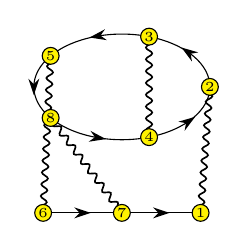
\begin{tikzpicture}
    \def \R {0.8}
    \def \ratio {0.5}
    \tikzstyle{every node}=[draw, fill=yellow, circle,inner sep=.5pt,font=\tiny];
    \begin{scope}[yshift= -\R cm, scale=1, xscale = -1]
    \coordinate (a3) at (0.0000, 0);
    \coordinate (a2) at (1.0000, 0);
    \coordinate (a1) at (-1.0000, 0);
    \draw[bareG] (a3) -- (a1);
    \draw[bareG] (a2) -- (a3);
    \end{scope}
    \begin{scope}[xshift=0.0000*\R cm, yshift =1.0000*\R cm, yscale=0.6]
    \def \n {5}
    \def \r {2.2361*\ratio cm}
    \def \twist {0}
    \foreach \s in {1,...,\n}{
    \draw[bareG] ({360/\n * (\s - 1)+\twist}:\r) arc ({360/\n * (\s - 1)+\twist}:{360/\n * (\s)+\twist}:\r);}
    \coordinate (b1) at ({360/\n *(0)+\twist}:\r);
    \coordinate (b2) at ({360/\n *(1)+\twist}:\r);
    \coordinate (b3) at ({360/\n *(2)+\twist}:\r);
    \coordinate (b4) at ({360/\n *(3)+\twist}:\r);
    \coordinate (b5) at ({360/\n *(4)+\twist}:\r);
    \end{scope}
    \draw[bareU] (a1) -- (b1);
    \draw[bareU] (a2) -- (b3);
    \draw[bareU] (a3) -- (b4);
    \draw[bareU] (b2) -- (b5);
    \node at (a1){$1$};
    \node at (a2){$6$};
    \node at (a3){$7$};
    \node at (b1){$2$};
    \node at (b2){$3$};
    \node at (b3){$5$};
    \node at (b4){$8$};
    \node at (b5){$4$};
    \end{tikzpicture}
    &
    
    
    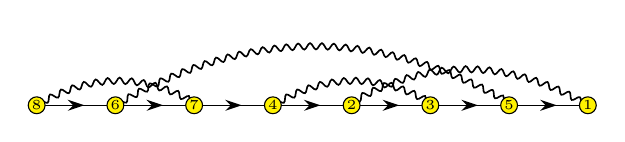
\begin{tikzpicture}
    \def \R {0.8}
    \def \ratio {0.5}
    \tikzstyle{every node}=[draw, fill=yellow, circle,inner sep=.5pt,font=\tiny];
    \begin{scope}[yshift= -\R cm, scale=1, xscale = -1]
    \coordinate (a8) at (-2.5000, 0);
    \coordinate (a7) at (-1.5000, 0);
    \coordinate (a6) at (-0.5000, 0);
    \coordinate (a5) at (0.5000, 0);
    \coordinate (a4) at (1.5000, 0);
    \coordinate (a3) at (2.5000, 0);
    \coordinate (a2) at (3.5000, 0);
    \coordinate (a1) at (-3.5000, 0);
    \draw[bareG] (a8) -- (a1);
    \draw[bareU] (a1) to [bend left] (a6);
    \draw[bareG] (a2) -- (a3);
    \draw[bareU] (a2) to [bend right] (a4);
    \draw[bareG] (a3) -- (a4);
    \draw[bareU] (a3) to [bend right] (a8);
    \draw[bareG] (a4) -- (a5);
    \draw[bareG] (a5) -- (a6);
    \draw[bareU] (a5) to [bend right] (a7);
    \draw[bareG] (a6) -- (a7);
    \draw[bareG] (a7) -- (a8);
    \end{scope}
    \node at (a1){$1$};
    \node at (a2){$8$};
    \node at (a3){$6$};
    \node at (a4){$7$};
    \node at (a5){$4$};
    \node at (a6){$2$};
    \node at (a7){$3$};
    \node at (a8){$5$};
    \end{tikzpicture}
    &
    
    
    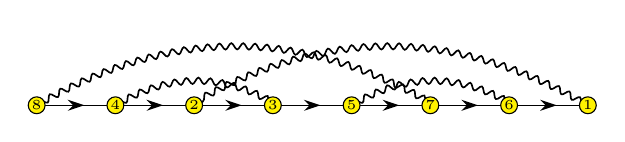
\begin{tikzpicture}
    \def \R {0.8}
    \def \ratio {0.5}
    \tikzstyle{every node}=[draw, fill=yellow, circle,inner sep=.5pt,font=\tiny];
    \begin{scope}[yshift= -\R cm, scale=1, xscale = -1]
    \coordinate (a8) at (-2.5000, 0);
    \coordinate (a7) at (-1.5000, 0);
    \coordinate (a6) at (-0.5000, 0);
    \coordinate (a5) at (0.5000, 0);
    \coordinate (a4) at (1.5000, 0);
    \coordinate (a3) at (2.5000, 0);
    \coordinate (a2) at (3.5000, 0);
    \coordinate (a1) at (-3.5000, 0);
    \draw[bareG] (a8) -- (a1);
    \draw[bareU] (a1) to [bend left] (a4);
    \draw[bareG] (a2) -- (a3);
    \draw[bareU] (a2) to [bend right] (a7);
    \draw[bareG] (a3) -- (a4);
    \draw[bareU] (a3) to [bend right] (a5);
    \draw[bareG] (a4) -- (a5);
    \draw[bareG] (a5) -- (a6);
    \draw[bareG] (a6) -- (a7);
    \draw[bareU] (a6) to [bend right] (a8);
    \draw[bareG] (a7) -- (a8);
    \end{scope}
    \node at (a1){$1$};
    \node at (a2){$8$};
    \node at (a3){$4$};
    \node at (a4){$2$};
    \node at (a5){$3$};
    \node at (a6){$5$};
    \node at (a7){$7$};
    \node at (a8){$6$};
    \end{tikzpicture}
    &
    
    
    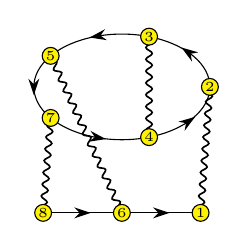
\begin{tikzpicture}
    \def \R {0.8}
    \def \ratio {0.5}
    \tikzstyle{every node}=[draw, fill=yellow, circle,inner sep=.5pt,font=\tiny];
    \begin{scope}[yshift= -\R cm, scale=1, xscale = -1]
    \coordinate (a3) at (0.0000, 0);
    \coordinate (a2) at (1.0000, 0);
    \coordinate (a1) at (-1.0000, 0);
    \draw[bareG] (a3) -- (a1);
    \draw[bareG] (a2) -- (a3);
    \end{scope}
    \begin{scope}[xshift=0.0000*\R cm, yshift =1.0000*\R cm, yscale=0.6]
    \def \n {5}
    \def \r {2.2361*\ratio cm}
    \def \twist {0}
    \foreach \s in {1,...,\n}{
    \draw[bareG] ({360/\n * (\s - 1)+\twist}:\r) arc ({360/\n * (\s - 1)+\twist}:{360/\n * (\s)+\twist}:\r);}
    \coordinate (b1) at ({360/\n *(0)+\twist}:\r);
    \coordinate (b2) at ({360/\n *(1)+\twist}:\r);
    \coordinate (b3) at ({360/\n *(2)+\twist}:\r);
    \coordinate (b4) at ({360/\n *(3)+\twist}:\r);
    \coordinate (b5) at ({360/\n *(4)+\twist}:\r);
    \end{scope}
    \draw[bareU] (a1) -- (b1);
    \draw[bareU] (a2) -- (b4);
    \draw[bareU] (a3) -- (b3);
    \draw[bareU] (b2) -- (b5);
    \node at (a1){$1$};
    \node at (a2){$8$};
    \node at (a3){$6$};
    \node at (b1){$2$};
    \node at (b2){$3$};
    \node at (b3){$5$};
    \node at (b4){$7$};
    \node at (b5){$4$};
    \end{tikzpicture}
    &
    
    
    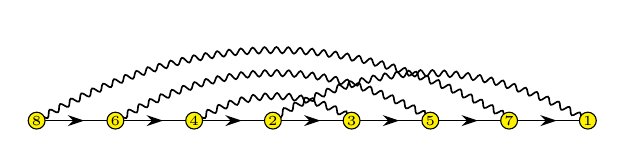
\begin{tikzpicture}
    \def \R {0.8}
    \def \ratio {0.5}
    \tikzstyle{every node}=[draw, fill=yellow, circle,inner sep=.5pt,font=\tiny];
    \begin{scope}[yshift= -\R cm, scale=1, xscale = -1]
    \coordinate (a8) at (-2.5000, 0);
    \coordinate (a7) at (-1.5000, 0);
    \coordinate (a6) at (-0.5000, 0);
    \coordinate (a5) at (0.5000, 0);
    \coordinate (a4) at (1.5000, 0);
    \coordinate (a3) at (2.5000, 0);
    \coordinate (a2) at (3.5000, 0);
    \coordinate (a1) at (-3.5000, 0);
    \draw[bareG] (a8) -- (a1);
    \draw[bareU] (a1) to [bend left] (a5);
    \draw[bareG] (a2) -- (a3);
    \draw[bareU] (a2) to [bend right] (a8);
    \draw[bareG] (a3) -- (a4);
    \draw[bareU] (a3) to [bend right] (a7);
    \draw[bareG] (a4) -- (a5);
    \draw[bareU] (a4) to [bend right] (a6);
    \draw[bareG] (a5) -- (a6);
    \draw[bareG] (a6) -- (a7);
    \draw[bareG] (a7) -- (a8);
    \end{scope}
    \node at (a1){$1$};
    \node at (a2){$8$};
    \node at (a3){$6$};
    \node at (a4){$4$};
    \node at (a5){$2$};
    \node at (a6){$3$};
    \node at (a7){$5$};
    \node at (a8){$7$};
    \end{tikzpicture}
    &
    
    
    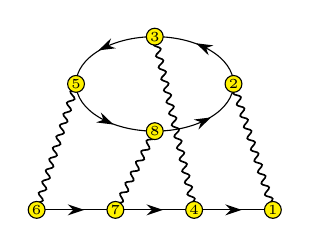
\begin{tikzpicture}
    \def \R {0.8}
    \def \ratio {0.5}
    \tikzstyle{every node}=[draw, fill=yellow, circle,inner sep=.5pt,font=\tiny];
    \begin{scope}[yshift= -\R cm, scale=1, xscale = -1]
    \coordinate (a4) at (-0.5000, 0);
    \coordinate (a3) at (0.5000, 0);
    \coordinate (a2) at (1.5000, 0);
    \coordinate (a1) at (-1.5000, 0);
    \draw[bareG] (a4) -- (a1);
    \draw[bareG] (a2) -- (a3);
    \draw[bareG] (a3) -- (a4);
    \end{scope}
    \begin{scope}[xshift=0.0000*\R cm, yshift =1.0000*\R cm, yscale=0.6]
    \def \n {4}
    \def \r {2.0000*\ratio cm}
    \def \twist {0}
    \foreach \s in {1,...,\n}{
    \draw[bareG] ({360/\n * (\s - 1)+\twist}:\r) arc ({360/\n * (\s - 1)+\twist}:{360/\n * (\s)+\twist}:\r);}
    \coordinate (b1) at ({360/\n *(0)+\twist}:\r);
    \coordinate (b2) at ({360/\n *(1)+\twist}:\r);
    \coordinate (b3) at ({360/\n *(2)+\twist}:\r);
    \coordinate (b4) at ({360/\n *(3)+\twist}:\r);
    \end{scope}
    \draw[bareU] (a1) -- (b1);
    \draw[bareU] (a2) -- (b3);
    \draw[bareU] (a3) -- (b4);
    \draw[bareU] (a4) -- (b2);
    \node at (a1){$1$};
    \node at (a2){$6$};
    \node at (a3){$7$};
    \node at (a4){$4$};
    \node at (b1){$2$};
    \node at (b2){$3$};
    \node at (b3){$5$};
    \node at (b4){$8$};
    \end{tikzpicture}
    &
    
    
    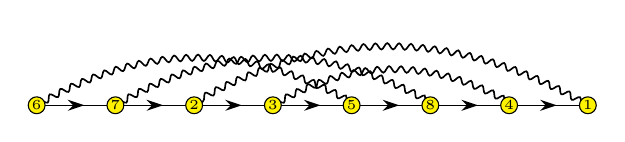
\begin{tikzpicture}
    \def \R {0.8}
    \def \ratio {0.5}
    \tikzstyle{every node}=[draw, fill=yellow, circle,inner sep=.5pt,font=\tiny];
    \begin{scope}[yshift= -\R cm, scale=1, xscale = -1]
    \coordinate (a8) at (-2.5000, 0);
    \coordinate (a7) at (-1.5000, 0);
    \coordinate (a6) at (-0.5000, 0);
    \coordinate (a5) at (0.5000, 0);
    \coordinate (a4) at (1.5000, 0);
    \coordinate (a3) at (2.5000, 0);
    \coordinate (a2) at (3.5000, 0);
    \coordinate (a1) at (-3.5000, 0);
    \draw[bareG] (a8) -- (a1);
    \draw[bareU] (a1) to [bend left] (a4);
    \draw[bareG] (a2) -- (a3);
    \draw[bareU] (a2) to [bend right] (a6);
    \draw[bareG] (a3) -- (a4);
    \draw[bareU] (a3) to [bend right] (a7);
    \draw[bareG] (a4) -- (a5);
    \draw[bareG] (a5) -- (a6);
    \draw[bareU] (a5) to [bend right] (a8);
    \draw[bareG] (a6) -- (a7);
    \draw[bareG] (a7) -- (a8);
    \end{scope}
    \node at (a1){$1$};
    \node at (a2){$6$};
    \node at (a3){$7$};
    \node at (a4){$2$};
    \node at (a5){$3$};
    \node at (a6){$5$};
    \node at (a7){$8$};
    \node at (a8){$4$};
    \end{tikzpicture}
    &
    
    
    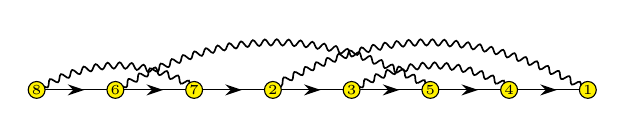
\begin{tikzpicture}
    \def \R {0.8}
    \def \ratio {0.5}
    \tikzstyle{every node}=[draw, fill=yellow, circle,inner sep=.5pt,font=\tiny];
    \begin{scope}[yshift= -\R cm, scale=1, xscale = -1]
    \coordinate (a8) at (-2.5000, 0);
    \coordinate (a7) at (-1.5000, 0);
    \coordinate (a6) at (-0.5000, 0);
    \coordinate (a5) at (0.5000, 0);
    \coordinate (a4) at (1.5000, 0);
    \coordinate (a3) at (2.5000, 0);
    \coordinate (a2) at (3.5000, 0);
    \coordinate (a1) at (-3.5000, 0);
    \draw[bareG] (a8) -- (a1);
    \draw[bareU] (a1) to [bend left] (a5);
    \draw[bareG] (a2) -- (a3);
    \draw[bareU] (a2) to [bend right] (a4);
    \draw[bareG] (a3) -- (a4);
    \draw[bareU] (a3) to [bend right] (a7);
    \draw[bareG] (a4) -- (a5);
    \draw[bareG] (a5) -- (a6);
    \draw[bareG] (a6) -- (a7);
    \draw[bareU] (a6) to [bend right] (a8);
    \draw[bareG] (a7) -- (a8);
    \end{scope}
    \node at (a1){$1$};
    \node at (a2){$8$};
    \node at (a3){$6$};
    \node at (a4){$7$};
    \node at (a5){$2$};
    \node at (a6){$3$};
    \node at (a7){$5$};
    \node at (a8){$4$};
    \end{tikzpicture}
    &
    
    
    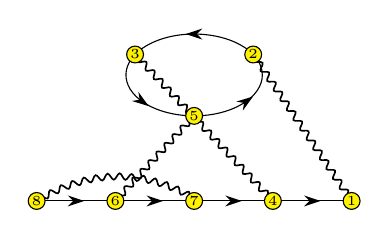
\begin{tikzpicture}
    \def \R {0.8}
    \def \ratio {0.5}
    \tikzstyle{every node}=[draw, fill=yellow, circle,inner sep=.5pt,font=\tiny];
    \begin{scope}[yshift= -\R cm, scale=1, xscale = -1]
    \coordinate (a5) at (-1.0000, 0);
    \coordinate (a4) at (0.0000, 0);
    \coordinate (a3) at (1.0000, 0);
    \coordinate (a2) at (2.0000, 0);
    \coordinate (a1) at (-2.0000, 0);
    \draw[bareG] (a5) -- (a1);
    \draw[bareG] (a2) -- (a3);
    \draw[bareU] (a2) to [bend right] (a4);
    \draw[bareG] (a3) -- (a4);
    \draw[bareG] (a4) -- (a5);
    \end{scope}
    \begin{scope}[xshift=0.0000*\R cm, yshift =1.0000*\R cm, yscale=0.6]
    \def \n {3}
    \def \r {1.7321*\ratio cm}
    \def \twist {30}
    \foreach \s in {1,...,\n}{
    \draw[bareG] ({360/\n * (\s - 1)+\twist}:\r) arc ({360/\n * (\s - 1)+\twist}:{360/\n * (\s)+\twist}:\r);}
    \coordinate (b1) at ({360/\n *(0)+\twist}:\r);
    \coordinate (b2) at ({360/\n *(1)+\twist}:\r);
    \coordinate (b3) at ({360/\n *(2)+\twist}:\r);
    \end{scope}
    \draw[bareU] (a1) -- (b1);
    \draw[bareU] (a3) -- (b3);
    \draw[bareU] (a5) -- (b2);
    \node at (a1){$1$};
    \node at (a2){$8$};
    \node at (a3){$6$};
    \node at (a4){$7$};
    \node at (a5){$4$};
    \node at (b1){$2$};
    \node at (b2){$3$};
    \node at (b3){$5$};
    \end{tikzpicture}
    &
    
    
    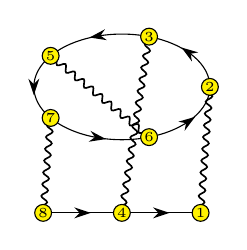
\begin{tikzpicture}
    \def \R {0.8}
    \def \ratio {0.5}
    \tikzstyle{every node}=[draw, fill=yellow, circle,inner sep=.5pt,font=\tiny];
    \begin{scope}[yshift= -\R cm, scale=1, xscale = -1]
    \coordinate (a3) at (0.0000, 0);
    \coordinate (a2) at (1.0000, 0);
    \coordinate (a1) at (-1.0000, 0);
    \draw[bareG] (a3) -- (a1);
    \draw[bareG] (a2) -- (a3);
    \end{scope}
    \begin{scope}[xshift=0.0000*\R cm, yshift =1.0000*\R cm, yscale=0.6]
    \def \n {5}
    \def \r {2.2361*\ratio cm}
    \def \twist {0}
    \foreach \s in {1,...,\n}{
    \draw[bareG] ({360/\n * (\s - 1)+\twist}:\r) arc ({360/\n * (\s - 1)+\twist}:{360/\n * (\s)+\twist}:\r);}
    \coordinate (b1) at ({360/\n *(0)+\twist}:\r);
    \coordinate (b2) at ({360/\n *(1)+\twist}:\r);
    \coordinate (b3) at ({360/\n *(2)+\twist}:\r);
    \coordinate (b4) at ({360/\n *(3)+\twist}:\r);
    \coordinate (b5) at ({360/\n *(4)+\twist}:\r);
    \end{scope}
    \draw[bareU] (a1) -- (b1);
    \draw[bareU] (a2) -- (b4);
    \draw[bareU] (a3) -- (b2);
    \draw[bareU] (b3) -- (b5);
    \node at (a1){$1$};
    \node at (a2){$8$};
    \node at (a3){$4$};
    \node at (b1){$2$};
    \node at (b2){$3$};
    \node at (b3){$5$};
    \node at (b4){$7$};
    \node at (b5){$6$};
    \end{tikzpicture}
    &
    
    
    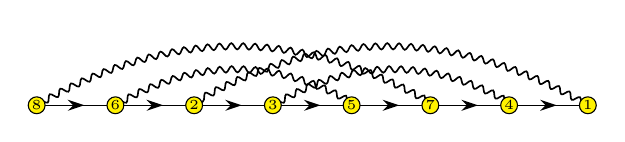
\begin{tikzpicture}
    \def \R {0.8}
    \def \ratio {0.5}
    \tikzstyle{every node}=[draw, fill=yellow, circle,inner sep=.5pt,font=\tiny];
    \begin{scope}[yshift= -\R cm, scale=1, xscale = -1]
    \coordinate (a8) at (-2.5000, 0);
    \coordinate (a7) at (-1.5000, 0);
    \coordinate (a6) at (-0.5000, 0);
    \coordinate (a5) at (0.5000, 0);
    \coordinate (a4) at (1.5000, 0);
    \coordinate (a3) at (2.5000, 0);
    \coordinate (a2) at (3.5000, 0);
    \coordinate (a1) at (-3.5000, 0);
    \draw[bareG] (a8) -- (a1);
    \draw[bareU] (a1) to [bend left] (a4);
    \draw[bareG] (a2) -- (a3);
    \draw[bareU] (a2) to [bend right] (a7);
    \draw[bareG] (a3) -- (a4);
    \draw[bareU] (a3) to [bend right] (a6);
    \draw[bareG] (a4) -- (a5);
    \draw[bareG] (a5) -- (a6);
    \draw[bareU] (a5) to [bend right] (a8);
    \draw[bareG] (a6) -- (a7);
    \draw[bareG] (a7) -- (a8);
    \end{scope}
    \node at (a1){$1$};
    \node at (a2){$8$};
    \node at (a3){$6$};
    \node at (a4){$2$};
    \node at (a5){$3$};
    \node at (a6){$5$};
    \node at (a7){$7$};
    \node at (a8){$4$};
    \end{tikzpicture}
    &
    
    
    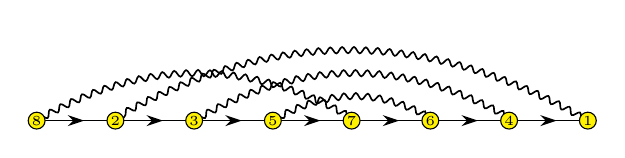
\begin{tikzpicture}
    \def \R {0.8}
    \def \ratio {0.5}
    \tikzstyle{every node}=[draw, fill=yellow, circle,inner sep=.5pt,font=\tiny];
    \begin{scope}[yshift= -\R cm, scale=1, xscale = -1]
    \coordinate (a8) at (-2.5000, 0);
    \coordinate (a7) at (-1.5000, 0);
    \coordinate (a6) at (-0.5000, 0);
    \coordinate (a5) at (0.5000, 0);
    \coordinate (a4) at (1.5000, 0);
    \coordinate (a3) at (2.5000, 0);
    \coordinate (a2) at (3.5000, 0);
    \coordinate (a1) at (-3.5000, 0);
    \draw[bareG] (a8) -- (a1);
    \draw[bareU] (a1) to [bend left] (a3);
    \draw[bareG] (a2) -- (a3);
    \draw[bareU] (a2) to [bend right] (a6);
    \draw[bareG] (a3) -- (a4);
    \draw[bareG] (a4) -- (a5);
    \draw[bareU] (a4) to [bend right] (a8);
    \draw[bareG] (a5) -- (a6);
    \draw[bareU] (a5) to [bend right] (a7);
    \draw[bareG] (a6) -- (a7);
    \draw[bareG] (a7) -- (a8);
    \end{scope}
    \node at (a1){$1$};
    \node at (a2){$8$};
    \node at (a3){$2$};
    \node at (a4){$3$};
    \node at (a5){$5$};
    \node at (a6){$7$};
    \node at (a7){$6$};
    \node at (a8){$4$};
    \end{tikzpicture}
    &
    
    
    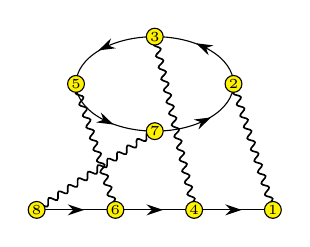
\begin{tikzpicture}
    \def \R {0.8}
    \def \ratio {0.5}
    \tikzstyle{every node}=[draw, fill=yellow, circle,inner sep=.5pt,font=\tiny];
    \begin{scope}[yshift= -\R cm, scale=1, xscale = -1]
    \coordinate (a4) at (-0.5000, 0);
    \coordinate (a3) at (0.5000, 0);
    \coordinate (a2) at (1.5000, 0);
    \coordinate (a1) at (-1.5000, 0);
    \draw[bareG] (a4) -- (a1);
    \draw[bareG] (a2) -- (a3);
    \draw[bareG] (a3) -- (a4);
    \end{scope}
    \begin{scope}[xshift=0.0000*\R cm, yshift =1.0000*\R cm, yscale=0.6]
    \def \n {4}
    \def \r {2.0000*\ratio cm}
    \def \twist {0}
    \foreach \s in {1,...,\n}{
    \draw[bareG] ({360/\n * (\s - 1)+\twist}:\r) arc ({360/\n * (\s - 1)+\twist}:{360/\n * (\s)+\twist}:\r);}
    \coordinate (b1) at ({360/\n *(0)+\twist}:\r);
    \coordinate (b2) at ({360/\n *(1)+\twist}:\r);
    \coordinate (b3) at ({360/\n *(2)+\twist}:\r);
    \coordinate (b4) at ({360/\n *(3)+\twist}:\r);
    \end{scope}
    \draw[bareU] (a1) -- (b1);
    \draw[bareU] (a2) -- (b4);
    \draw[bareU] (a3) -- (b3);
    \draw[bareU] (a4) -- (b2);
    \node at (a1){$1$};
    \node at (a2){$8$};
    \node at (a3){$6$};
    \node at (a4){$4$};
    \node at (b1){$2$};
    \node at (b2){$3$};
    \node at (b3){$5$};
    \node at (b4){$7$};
    \end{tikzpicture}  \\ [0.5ex] 
%    \hline
    \end{longtable}
    
\end{document}
